\documentclass[11pt,letterpaper]{article}

\usepackage{showlabels}
\usepackage{fullpage}
\usepackage{pslatex}
%\usepackage{latexsym}
\usepackage[english]{babel}
\usepackage[utf8]{inputenc}
\usepackage{amsmath}
\usepackage{bm}
%\usepackage{tikz}
\usepackage{xcolor}
\usepackage{url}
%\usepackage[colorinlistoftodos]{todonotes}
\usepackage{rotating}
\usepackage{natbib}
\usepackage{amssymb}
\usepackage{lingmacros}

\usepackage{CJKutf8}
\newcommand{\korean}[1]{\begin{CJK}{UTF8}{mj}#1\end{CJK}}

\usepackage{tikz}


\usepackage{colortbl}

%\usepackage{xeCJK}

\usepackage{natbib}
\bibliographystyle{unsrtnat}

%\usepackage{latexsym}
\usepackage[english]{babel}
\usepackage[utf8]{inputenc}
\usepackage{bm}
\usepackage{graphicx}
%\usepackage{tikz}
\usepackage{xcolor}
\usepackage{url}
%\usepackage[colorinlistoftodos]{todonotes}
\usepackage{rotating}
\usepackage{multirow}


%\usepackage{linguex}
%\usepackage{lingmacros}


\usepackage{hyperref}

\usepackage{tikz-dependency}
\usepackage{changepage}
\usepackage{longtable}


\newcommand{\R}[0]{\mathbb{R}}
\newcommand{\Prob}[0]{\mathbb{P}}
\newcommand{\Ff}[0]{\mathcal{F}}

\usepackage{multirow}

\newcommand{\soft}[1]{}
\newcommand{\nopreview}[1]{}
\newcommand\comment[1]{{\color{red}#1}}
\newcommand\mhahn[1]{{\color{red}(#1)}}
\newcommand\becky[1]{{\color{blue}(#1)}}
\newcommand\note[1]{{\color{red}(#1)}}
\newcommand\jd[1]{{\color{red}(#1)}}
\newcommand\rljf[1]{{\color{red}(#1)}}
\newcommand{\key}[1]{\textbf{#1}}

\DeclareMathOperator*{\argmax}{arg\,max}
\DeclareMathOperator*{\argmin}{arg\,min}
\DeclareMathOperator{\E}{\mathop{\mathbb{E}}}



\usepackage{amsthm}

\newcommand{\thetad}[0]{{\theta-d}}
\newcommand{\thetal}[0]{{\theta-{LM}}}

\newcounter{theorem}
\newtheorem{proposition}[theorem]{Proposition}
\newtheorem{thm}[theorem]{Theorem}
\newtheorem{corollary}[theorem]{Corollary}
\newtheorem{question}[theorem]{Question}
\newtheorem{example}[theorem]{Example}
\newtheorem{defin}[theorem]{Definition}
\newtheorem{definition}[theorem]{Definition}
\newtheorem{lemma}[theorem]{Lemma}


%\usepackage{linguex}
%\newcommand{\key}[1]{\textbf{#1}}



\renewcommand{\thefigure}{S\arabic{figure}}
\renewcommand{\thetable}{S\arabic{table}}
\renewcommand{\thesection}{S\arabic{section}}

\newcommand{\utterance}{\mathcal{U}}
\newcommand{\tree}{\mathcal{T}}



\usepackage{siunitx}



\usepackage{longtable}



\frenchspacing
%\def\baselinestretch{0.975}

%\emnlpfinalcopy
%\def\emnlppaperid{496}

\title{Morpheme Ordering across Languages reflects optimization for memory efficiency / information locality}

\begin{document}

\maketitle

\begin{abstract}
    The order of morphemes in a word shows well-documented tendencies across languages.
    These have been explained in terms of notions such as semantic scope and relevance in prior work.
A recent theory (CITE) argues that word and morpheme order in language optimizes a tradeoff between Memory and surprisal, and provided initial evidence from twoi languages that morpheme order can partly be explained by optimization for this treadeoff.
    %Efficient memory--surprisal tradeoffs are achieved by orders that display information locality, whereby elements that have high mutual information are closer together.
    In this work, we test this idea more extensively using data from four additional agglutinative languages with significant amounts of morphology.
    
%    In this work, we examine corpus data from four languages to show that optimizing for tradeoff efficiency mostly predicts morpheme order in verb and noun morphology.
    
\end{abstract}


\section{Introduction}

Across languages, words are composed of morphemes, commonly defined as the smallest meaning-bearing units of language.
Morphemes can take different shapes.
In many cases, words can be segmented into a sequence of morphemes, as in the English word runners (root run-, derivation -er-, plural -s).
The order of morphemes within a word follows well-documented cross-linguistic tendencies, for instance, plural markers tend to be closer to noun stems than case markers \citep[112]{greenberg1963universals}.
These tendencies have been explained in terms of the relative scope of different morphemes  \citep{givon1971historical,venneman1973explanation,baker1985the,rice2000morpheme} and the strength of their semantic association with the root \citep{bybee-morphology-1985}.
%One family of explanations holds that those affixes are closest to the root that are most relevant to the root \citep{bybee-morphology-1985}.
%Other explanations suggest that morphemes are ordered based on (TODO CITE).

A recent theory proposes a cognitive explanation for these tendencies, arguing that ordering universals in language can be understood as arising from optimization of processing effort under memory limitations \citep{Hahn2020modeling}.
Formally, they introduced the notion of a memory-surprisal tradeoff: Depending on how many memory resources a comprehender invests, they can achieve different levels of surprisal.
(CITE) hypothesize that order of words and morphemes in language optimizes this tradeoff.
Optimizing the memory-surprisal tradeoff amounts to putting elements together when they predict each other strongly, as measured by mutual information.
In a case study, CITE apply this to morpheme ordering in Japanese and Sesotho, finding that optimization could partly reproduce morpheme ordering in these languages.
They also suggested that mutual information formalizes previous notions of strength of semantic association, such as \cite{bybee-morphology-1985}'s notion of \textit{relevance}.


In this work, we examine this theory on a broader basis by considering data from four additional languages.
We focus on languages where words tend to have multiple morphemes and these are mostly realized separately. Such languages are referred to as agglutinative (Greenberg 1954).
We obtained data from four languages (Korean, Turkish, Hungarian, Finnish).
Whereas \cite{Hahn2020modeling} only considered verb inflection, we also consider noun inflection across three languages.


%Greenberg 1963:  "the expression of number almost always comes between the noun base and the expression of case" (Greenberg 1963:112)

%Scope, Syntax, History
%Another family of explanations holds that morpheme ordering is to be explained diachronically, and that morpheme order reflects the order of independent words in earlier stages of a language.
%- Relevance, Proximity Principle, Iconicity




%Bybee on explanation:
%- regarding the historical explanation (Givon 1971, Vennemann 1973):
%Morphology is not always fossilizes syntax (Bybee and Brewer 1980, Bybee 1985 p. 39--40)


\section{Morpheme Ordering and Ordering Universals}

In this section, we introduce some general crosslinguistic tendencies in morpheme ordering, before discussing data from the six languages in Section XX.

\paragraph{Nouns}
Nouns commonly mark number and case.
For nouns, \citep[112]{greenberg1963universals} Universal 39 states that number affixes are closer to the stem than case affixes, if they appear on the same side.
In some languages, possession is also marked on the noun.

\paragraph{Verbs}
Verbs commonly mark a larger number of inflection categories.
Based on data from several dozens of languages, \citep{bybee-morphology-1985} proposes the following ordering of verb affixes:
\begin{quote}
\begin{tabular}{llllllllllllllllllllllllll}
verb stem & valence & voice & aspect & tense& mood & subject agreement
\end{tabular}
\end{quote}
\textit{Valence} affixes change the number of arguments; for instance, causatives add an argument (TODO example).
\textit{Voice} describes the distinction between active and passive.
\textit{Aspect} describes how an event unfolds over time, such as the English progressive -ing indicating that an action  is still ongoing.
\textit{Tense} describes where an event is located in time (e.g. past or future).
\textit{Mood} TODO
\textit{Subject person and number} mark categories of the subject, such as English third-person -s.

While these are particularly common types of affixes, there are further types.
Examples are polarity (negation), evidential (based on what evidence a speaker makes an assertion), and formality.


We focus on inflection, except in those cases where derivational affixes are clearly marked in available data.
Inflectional suffixes are generally outside of derivational affixes


\section{Background: Memory--Surprisal Tradeoff and Information Locality}

\citet{Hahn2020modeling} introduced the Memory--Surprisal Tradoff as a cognitive account of the order of words and morphemes in human language, based on a formalization of memory efficiency in incremental processing.

The memory-surprisal tradeoff links information-theoretic models of memory limitations with surprisal theory.
Surprisal theory \citep{hale2001probabilistic, levy2008expectation} states that the processing effort on a word $w_t$ in context $w-1 ... w_{t-1}$ is proportional to its surprisal
     \begin{equation}   \label{eq:true-surp}
    \text{Difficulty} \propto -\log P(w_t , w_1\dots w_{t-1}).
\end{equation}
Surprisal as estimated by corpus-based methods is a successful predictor of reading time on naturalistic text \citep{smith2013effect,goodkind-predictive-2018,frank2019interaction,aurnhammer2019evaluating,wilcox2020predictive}.
This effect can be explained in terms of mechanisms such as preactivation and integration~\citep{kuperberg2016we}.
However, due to limitations in human memory, human expectations in reality do not reflect the true context $w-1\dots w_{t-1}$, but some memory representation $m\_t$:
\begin{equation}   \label{eq:lossy-surp}
    \text{Difficulty} \propto -\log P(w_t | m_t).
\end{equation}
\citet{Hahn2020modeling} note that there is a tradeoff between average surprisal and memory capacity:
The more information a listener stores in $m\_t$, the lower their surprisal will be on average.
This is because higher precision of memory leads to more precise expectations, which will achiever lower surprisal on average.
More formally, given a function $M$ encoding contexts $w_1\dots w_{t_1}$ into memory representations $m_t$, there is a tradeoff between, on the one hand, the average surprisal $S\_M$, obtained by averaging $\log P(w_t , m_t)$ across the words in a text, and the memory capacity $H_M$, formalized as the average number of bits required to encode $m_t$.


\citet{Hahn2020modeling} prove a theorem that provides a method of estimating the memory-surprisal tradeoff from corpus data.
This theorem is based on \key{mutual information}, which quantifies the amount of statistical association between two random variables.
If $X, Z, Y$ are random variables, then the mutual information of $X$ and $Y$, conditioned on $Z$, is defined to be:
\begin{align}
\label{eq:mi}
    \operatorname{I}[X:Y,Z] &\equiv \sum_{x,y,z} P(x,y,z) \log \frac{P(x,y,z)}{P(x,z)P(y,z)}. % \text{ bits} \\
    %\nonumber
    %&= \operatorname{H}[X,Z] - \operatorname{H}[X,Y,Z] \\
    %\nonumber
    %&= \operatorname{H}[Y,Z] - \operatorname{H}[Y,X,Z].
\end{align}
The key quantity derived from this is the mutual information between elements (such as morphemes) that are some distance $t$, conditioned on the intervening elements:
\begin{equation*}
    I_t \equiv \operatorname{I}[w_t : w_0 , w_1, \dots, w_{t-1}].
\end{equation*}
Based on this notion, \citet{Hahn2020modeling}  prove the following bound on the memory-surprisal tradeoff ($S_\infty$ is the average surprisal that would be achieved with perfectly veridical memory representations):
\begin{thm}\label{prop:suboptimal}(Information locality bound, \citet{Hahn2020modeling})
For any positive integer $T$, let $M$ be a memory encoding function such that
\begin{equation}
\label{eq:memory-bound}
H_M \le \sum_{t=1}^T t I_t.
\end{equation}
Then we have a lower bound on the average surprisal under the memory encoding function $M$:
\begin{equation}
\label{eq:surprisal-bound}
S_M \ge S_\infty + \sum_{t=T+1}^\infty I_t.
\end{equation}
\end{thm}


A key consequence of this theorem is that it implies information locality:
Orderings optimize this tradeoff when elements with high mutual information are closer together.
A similar notion of information locality was previous derived by \citet{futrell2020lossy} for a specific family of memory representations $M$.
Information locality has had success as a predictor of word order \citep{futrell2019information}, in particular for universals of the order inside noun phrases \citep{culbertson2020from,hahn-information-theoretic-2018,DBLP:conf/acl/FutrellDS20}.

\citet{Hahn2020modeling} argue that information locality derives a range of locality principles proposed in the linguistic literature, including \cite{bybee-morphology-1985}'s idea that morphemes are closer together when they are more relevant to each other.
\mhahn{say more about relevance}

\section{Methods}

\subsection{Data} % TODO: Becky
% why agglutinative?

We are interested in analyzing languages in which words have easily separable morphemes and have a tendency to have more than two morphemes per word, because that allows us to vary morphemes distances. As such, we considered agglutinative languages that have morpheme-segmented corpora available. The language sample includes Universal Dependencies (UD) corpora for Japanese, Korean, Turkish, Hungarian, and Finnish (CITE). In addition, we use the Child Language Data Exchange System (CHILDES) Sesotho corpus (CITE). 

The Korean, Japanese, and Sesotho corpora have words segmented into the grapheme representations of their morphemes. However, the Turkish, Hungarian, and Finnish corpora do not segment the words into morphemes, but rather include a list of features (such as person, number, voice, etc.) present in each word. We built segmenters to reconstruct the order of morphemes in each word from those feature labels \becky{TODO: see Appendix?} \mhahn{Yes, I think we can explain in the main paper what data we collected in linguistic terms (e.g. finite verb forms, what we did with auxiliaries), and in the appendix discuss what steps were needed to do this. The technical details don't have to be 100\% there since the code will be available to the reviewers and readers.}.

The Sesotho and Japanese data was previously used by CITE; we reanalyze these data here in a way consistent across all six languages.

\begin{itemize}
    \item Grapheme, label, phoneme for Korean \mhahn{For now, I think we can place grapheme and phoneme versions into the appendix, and only discuss the MorphemeMeanings-based one in the main paper (i.e., ordering based on morpheme meanings, surprisal based on abstract morphemes, analogous to the Coarse+FineSurprisal version for the other languages.}
    For Korean, the corpus came with segmented morphemes labeled with fine-grained categories such as "ending final marker," or "predicative maker." We also built a segmenter to take in each segment and out
    \item Fine versus coarse for Turkish, Hungarian, Finnish \mhahn{In the main paper, I think it's enough to present the Coarse+FinalSurprisal results. We can present others in the appendix, and don't need to introduce them here in detail.}
\end{itemize}

\becky{discuss segmenters more} 

\subsection{Nouns}

\mhahn{Here is an idea for how we might structure this section: We can describe the systems in the individual languages in prose and in broad strokes here, highlighting what's common and what's different across languages. For the nouns, it's interesting to point out that the relative position of Case and Possessor differs between Finnish and the rest, whereas the position of Number is stable. For the verbs, the discussion could refer to Table~\ref{tab:table-orders}. I've collapsed all the Tense/Aspect/Modality/Negation morphemes into one big category ``TAM, Polarity'' since aligning the morphemes in each language with those individual categories seems very hard, and in any case there are differences between the languages. Talking about this in broad strokes, again highlighting parallels and differences, should be the right level of detail here. You can draw on Table S1 and Tables S5, S12, S13 in the appendix for my revised verb morpheme segmentation in Korean, Turkish, and Hungarian. We can then leave precise and detailed discussion of each of the languages, including detailed references to the literature for these individual languages, to the appendix. The \texttt{enumerate} blocks could go into the appendix, with some description of what each morpheme does and references to reference grammars (I can do this).}

We're interested in investigating languages where nouns are inflected with multiple suffixes, because that allows us to more extensively measure the relationship between mutual information and mutual information. As such, we only investigated our hypothesis on Turkish, Hungarian, and Finnish nouns. All of these languages inflect nouns for number, possessor person, possessor number, and case, in that order. Finnish is the exception, where we include derivation (verbs that are nominalized, for example), and where the possessor person and number appears after the case suffix in the natural ordering. 
In contrast, the number suffix, which is generally only marked for the plural, has a stable position close to the root in all three languages. Number has high mutual information with the noun root, because certain nouns have a tendency to appear only in the plural or only in the singular. As such, number must come close to the root. \becky{Is this correct? Also, should I move this?}
\mhahn{This is good. We could think about moving the part about mutual information up into a paragraph at the end of S3, where we could give the reader some intuition on why we expect MI to be a good predictor of ordering (as mentioned in my Slack message).}
\paragraph{Turkish Nouns}
\begin{enumerate}
    \item Number
    \item Possessor number and possessor person
    \item Case 
\end{enumerate}

\paragraph{Hungarian Nouns}
\url{https://cl.lingfil.uu.se/~bea/publ/megyesi-hungarian.pdf}
\begin{enumerate}
    \item Number
    \item Possessor person
    \item Possessor number \becky{Missing in citation}
    \item Case 
\end{enumerate}

\paragraph{Finnish Nouns}
\begin{enumerate}
    \item Derivation
    \item Number
    \item Case 
    \item Possessor person and possessor number
\end{enumerate}

\subsection{Verbs}
For verbs, we investigated Finnish, Hungarian, Japanese, Korean, Sesotho, and Turkish inflectional suffixes. Broadly speaking, all of the languages have a real ordering of valence, voice, negation, tense/aspect/mood (TAM), person and number, and formality, where applicable. \becky{Check that this is correct and discuss some specifics.} 

\begin{table}[]
    \centering
\begin{tabular}{l||l|l|l|l|l|l|llll}
                    & Turkish & Hungarian & Finnish  & Sesotho Pref.     & Ses Suff. & Japanese & Korean\\ \hline\hline
Derivation          &  &         &          &               & Reversive & suru    & ha,i\\ \hline
Valence             &  Causative &         &           & Object marker & Valence & Causative\\ \hline
Voice               & Passive & Passive    & Passive     &               & Passive & Passive\\ \hline
TAM, Pol.           & Negation  &   Potential  &   Tense/Asp &    Negation &  Politeness &      Potential        & Honorific \\
                    & Potential & Tense        &    Mood     &     Tense   &    Mood     &   Honorific  &    Tense       \\
                    &   TAM1    &          &                &         &                  & Tense/Aspect & Formality \\
                    & lar       &          &           &  & & Negation & Mood I\\
                    & TAM2         &           &               &          &       &      &  Mood II \\ \hline
Agreement           & Agreement & Agreement & Agreement & Agreement \\ \hline
\textit{Other}               & Formality          & Clitic    &              & Int/Rel &      &        & Politeness \\
                    &           &     &              &  &          &    & Conj \\
\end{tabular}
    \caption{Morpheme order across the six languages in our sample, matched with the universal order described by \cite{bybee-morphology-1985}.}
    \label{tab:table-orders}
\end{table}



\paragraph{Hungarian Verbs} \url{https://cl.lingfil.uu.se/~bea/publ/megyesi-hungarian.pdf}
\begin{enumerate}
    \item Voice \becky{Missing in citation}
    \item Mood
    \item Tense \mhahn{Potential mood appears in front of Tense, so I changed from Tense--Mood to Mood -- Tense as the order here.}
    \item Definiteness, person, and number: This suffix indicates the definiteness or indefiniteness of the direct object of the verb, as well as the person and number of the subject performing the verb. 
\end{enumerate}

\paragraph{Turkish Verbs}
\begin{enumerate}
    \item Voice
    \item Negation / polarity
    \item Aspect
    \item Evidential 
    \item Tense 
    \item Mood 
    \item Person and Number
    \item Formality
\end{enumerate}

\mhahn{I've changed this to the following}
\begin{enumerate}
    \item Valence (Causative -tir-)
    \item Voice (Passive -il-)
    \item Negation / polarity (Negation -ma-)
    \item Mood (Potential -bil-)
    \item TAM1: Tense, Aspect, Mood, Evidential
    \item 3rd Plural (-lar-)
    \item TAM2: Tense, Aspect, Mood, Evidential
    \item Subject agreement (incorporating TAM information)
    \item Formality (polite -makta-)
    \item Genitive (-dir-)
    \item Verbal Noun (-mak)
    \item Possessive agreement
\end{enumerate}




\paragraph{Finnish Verbs}
\begin{enumerate}
    \item Voice
    \item Tense 
    \item Mood 
    \item Person and number
    \item Clitic
\end{enumerate}


%https://en.wiktionary.org/wiki/%EB%B0%94%EB%9D%BC%EB%8B%A4

\section{Results}




\begin{figure}
    \centering
    \begin{tabular}{cccccc}
    Finnish & Turkish & Hungarian \\
        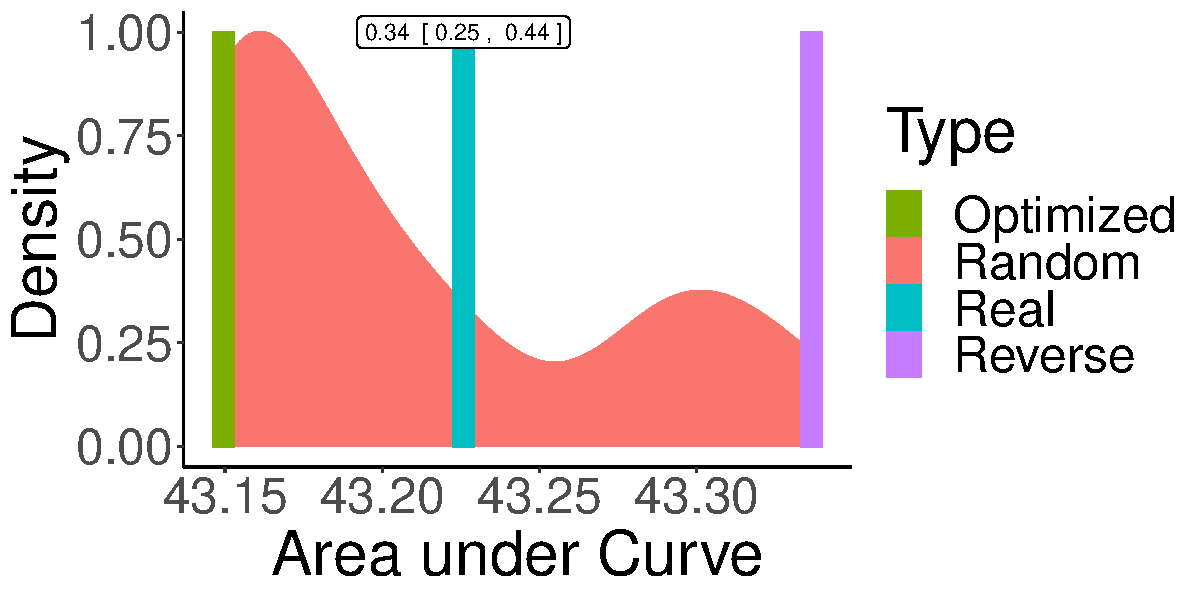
\includegraphics[width=0.3\textwidth]{figures/finnish_verbs/suffixes-byMorphemes-auc-hist-heldout-Coarse-FineSurprisal-optimized.pdf}
        &
    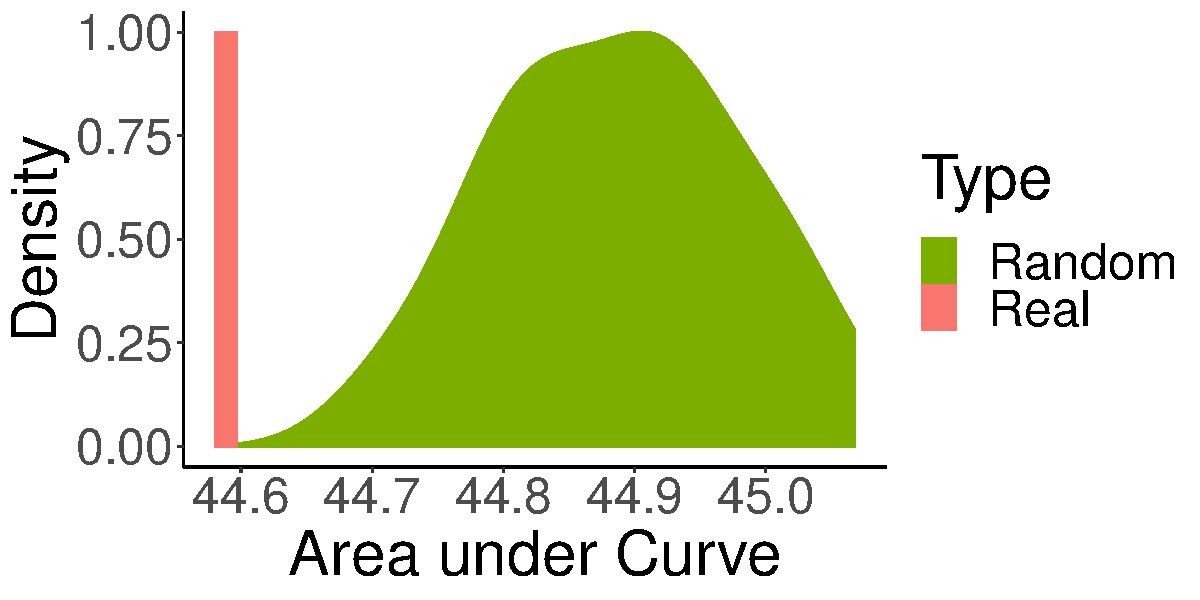
\includegraphics[width=0.3\textwidth]{figures/turkish_verbs/suffixes-byMorphemes-auc-hist-heldout-Coarse-FineSurprisal-optimized.pdf}
    &
    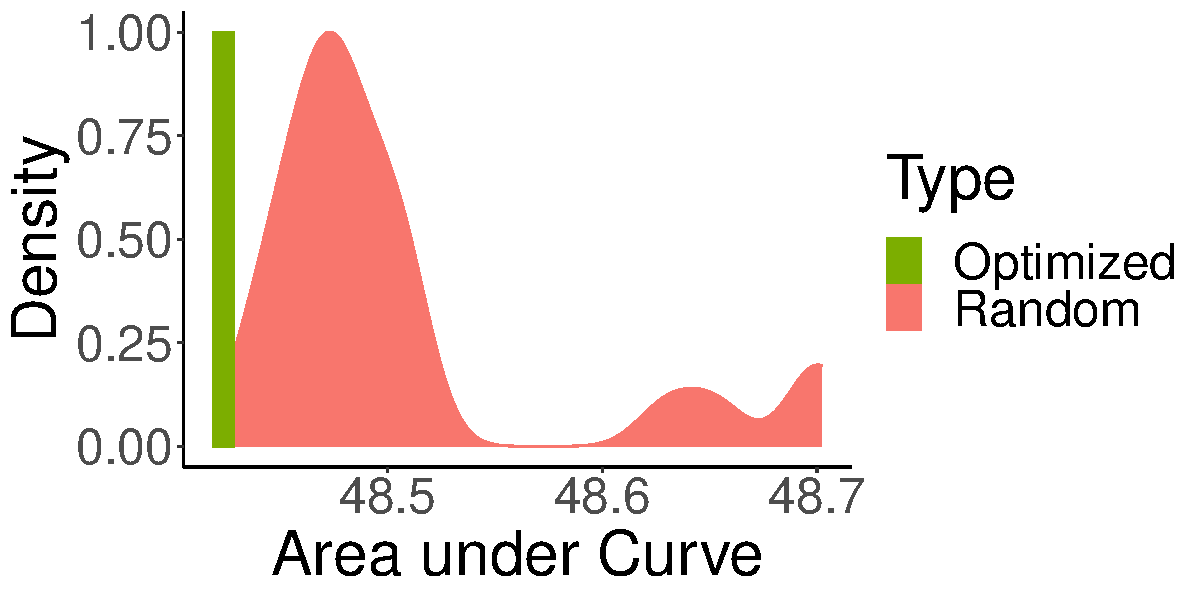
\includegraphics[width=0.3\textwidth]{figures/hungarian_verbs/suffixes-byMorphemes-auc-hist-heldout-Coarse-FineSurprisal-optimized.pdf}
    \\
    Korean & Japanese & Sesotho (prefixes) \\
    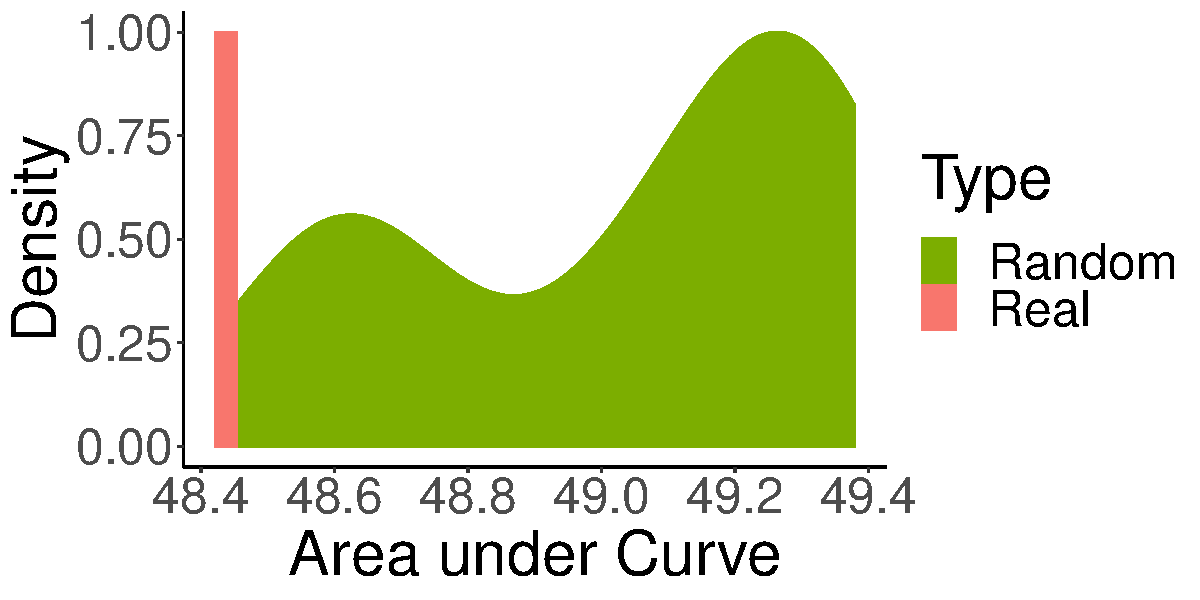
\includegraphics[width=0.3\textwidth]{figures/korean/suffixes-byMorphemes-auc-hist-heldout-Coarse-FineSurprisal-optimized.pdf}
    &
        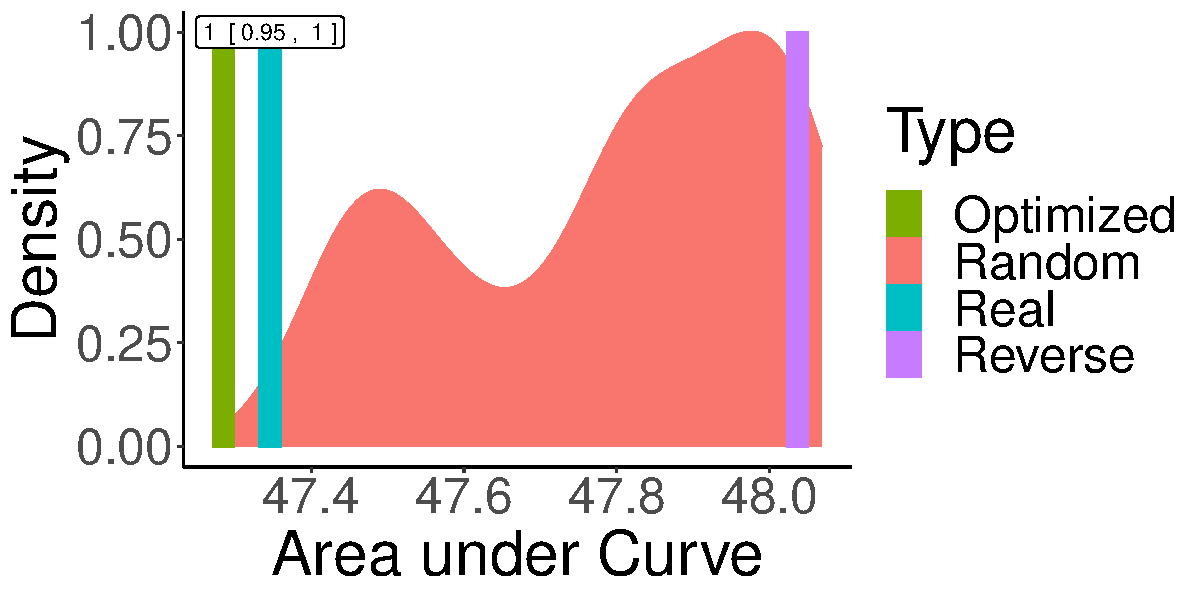
\includegraphics[width=0.3\textwidth]{figures/japanese/suffixes-byMorphemes-auc-hist-heldout-Coarse-FineSurprisal-optimized.pdf}
    \end{tabular}
%    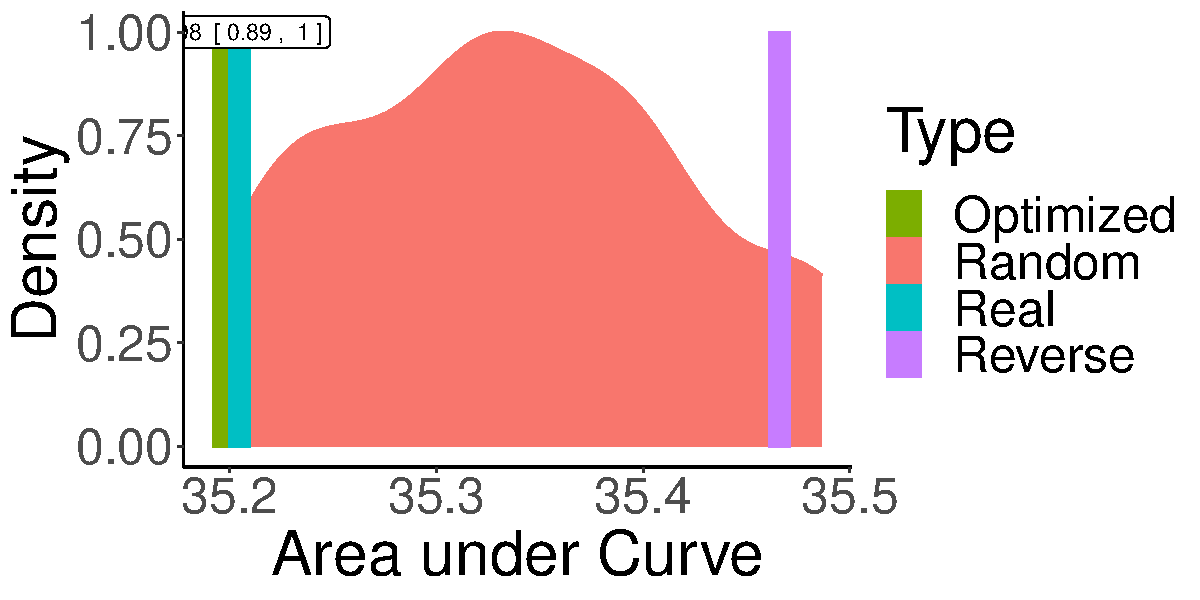
\includegraphics[width=0.2\textwidth]{figures/sesotho_prefixes/suffixes-byMorphemes-auc-hist-heldout-Coarse-FineSurprisal-optimized.pdf}
%    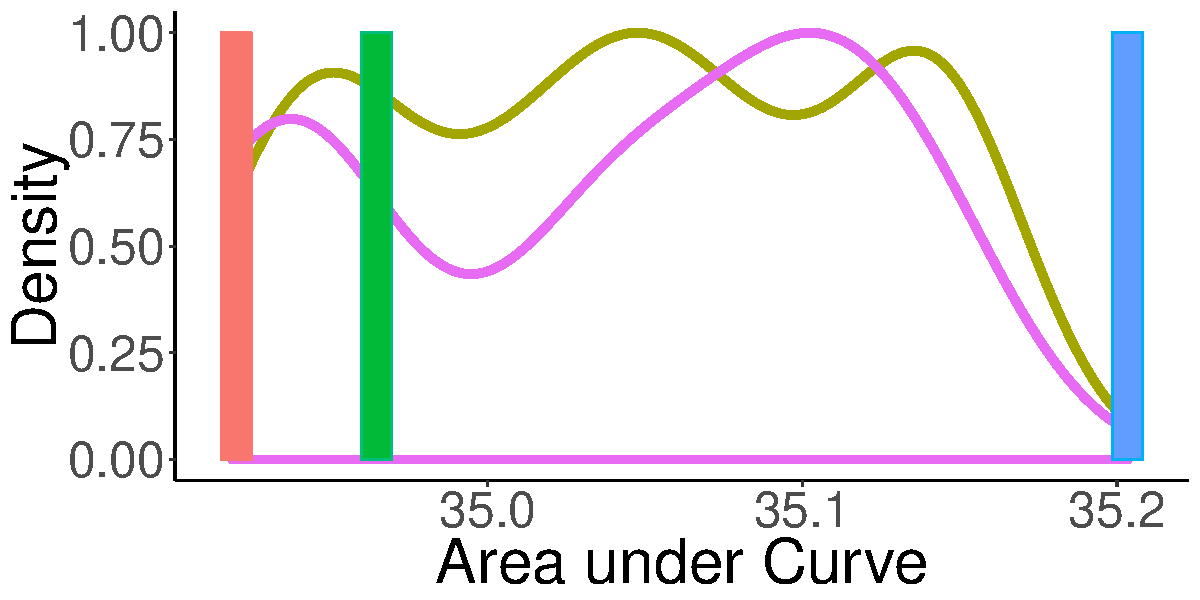
\includegraphics[width=0.2\textwidth]{figures/sesotho_suffixes/suffixes-byMorphemes-auc-hist-heldout-Coarse-FineSurprisal-optimized.pdf}
    \caption{Verb Suffixes}
    \label{fig:my-label}
\end{figure}


\begin{figure}
\begin{tabular}{ccc}
Finnish & Turkish & Hungarian \\
    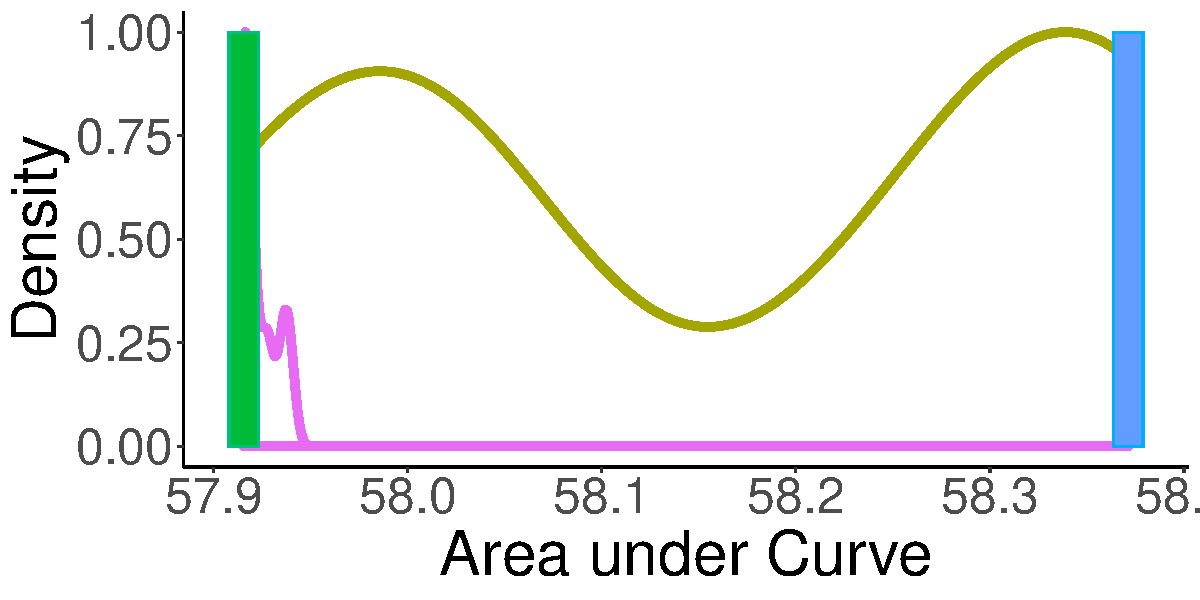
\includegraphics[width=0.3\textwidth]{figures/finnish_nouns/suffixes-byMorphemes-auc-hist-heldout-Coarse-FineSurprisal-optimized.pdf}
    &
    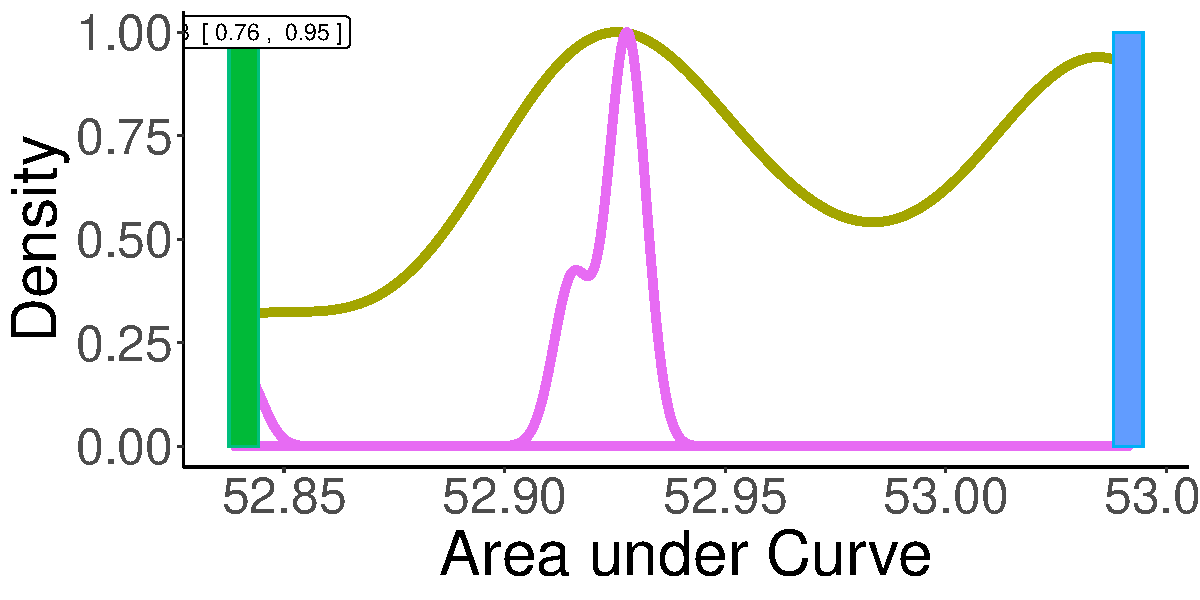
\includegraphics[width=0.3\textwidth]{figures/turkish_nouns/suffixes-byMorphemes-auc-hist-heldout-Coarse-FineSurprisal-optimized.pdf}
    &
    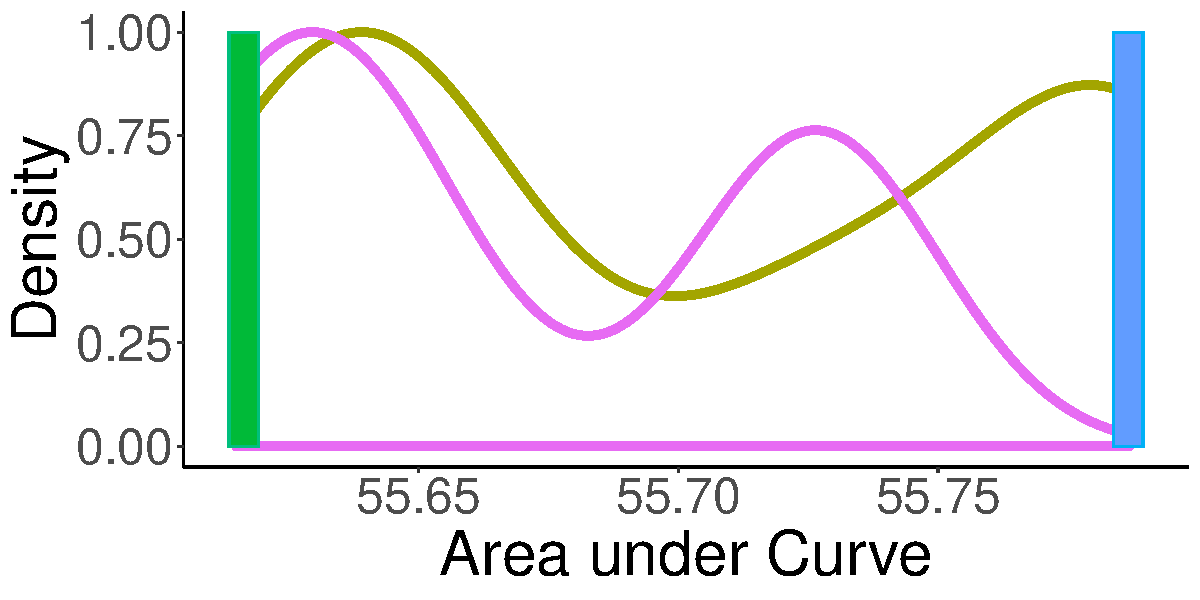
\includegraphics[width=0.3\textwidth]{figures/hungarian_nouns/suffixes-byMorphemes-auc-hist-heldout-Coarse-FineSurprisal-optimized.pdf}
    \end{tabular}
    \caption{Noun Suffixes}
    \label{fig:my-label}
\end{figure}

\begin{table}[]
    \centering
    \begin{tabular}{l|l|ll|lllllllll}
    &     &    \multicolumn{2}{c|}{Pairs} & \multicolumn{2}{c|}{Full} & \multicolumn{2}{c}{Full (Types)} \\
     &   &     Optim. & Baseline & Optim. & Baseline & Optim. & Baseline \\ \hline
Nouns & finnish nouns & 1.0 (0.0) & 0.42 (0.31) & 1.0 (0.0) & 0.37 (0.32) & 1.0 (0.0) & 0.38 (0.29) \\
 & turkish nouns & 1.0 (0.0) & 0.56 (0.36) & 1.0 (0.0) & 0.5 (0.37) & 1.0 (0.0) & 0.5 (0.36) \\
 & hungarian nouns & 1.0 (0.0) & 0.48 (0.22) & 1.0 (0.0) & 0.33 (0.27) & 1.0 (0.0) & 0.33 (0.27) \\ \hline
Verbs & finnish verbs & 0.4 (0.3) & 0.4 (0.37) & 0.38 (0.31) & 0.39 (0.38) & 0.36 (0.32) & 0.38 (0.37) \\
 & hungarian verbs & 0.95 (0.09) & 0.52 (0.37) & 0.95 (0.0) & 0.5 (0.4) & 0.94 (0.0) & 0.5 (0.39) \\
 & turkish verbs & 0.96 (0.09) & 0.46 (0.14) & 0.95 (0.0) & 0.37 (0.15) & 0.93 (0.07) & 0.36 (0.14) \\
 & korean & 0.97 (0.1) & 0.56 (0.33) & 0.97 (0.0) & 0.53 (0.33) & 0.95 (0.0) & 0.53 (0.36) \\
 & japanese & 0.94 (0.08) & 0.48 (0.24) & 0.93 (0.0) & 0.39 (0.24) & 0.9 (0.1) & 0.39 (0.24) \\
 & sesotho pre & -- & -- & -- & -- & -- & -- \\
 & sesotho suff & -- & -- & -- & -- & -- & -- \\

    \end{tabular}
    \caption{Accuracies in predicting morpheme ordering. `Optim.' indicates grammars optimized for AUC, `'Baseline' indicates randomly constructed weights.
    In each cell, we provide the mean and the stgandard deviation over orderings. `Pairs' indicates the fraction of pairs of morphemes occurring together in the same word that are ordered correctly. `Full' indicates the fraction of verb forms in the corpus that are ordered fully correctly. `Full (Types)' counts forms that occur multiple times only once, it thus down-weights the role of frequent forms.}
    \label{tab:my_label}
\end{table}



\begin{figure}[]
\begin{tabular}{cccccccc}
\textbf{Turkish} & \textbf{Hungarian} & \textbf{Finnish} \\
\begin{minipage}{.3\textwidth}
    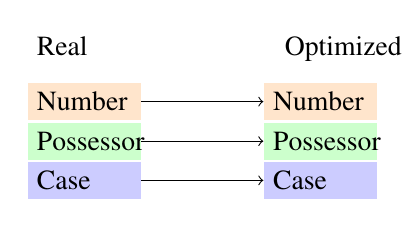
\begin{tikzpicture}[%
% common options for blocks:
block/.style = {draw, fill=blue!30, align=center, anchor=west,
            minimum height=0.65cm, inner sep=0},
% common options for the circles:
ball/.style = {circle, draw, align=center, anchor=north, inner sep=0}]
\node[rectangle,text width=1.2cm,anchor=base] (A0) at (1,-0.3) {Real};
\node[rectangle,text width=0.9cm,anchor=base] (B0) at (4,-0.3) {Optimized};
\node[rectangle,text width=1.2cm,anchor=base, fill=orange!20] (A1) at (1,-1.0) {Number};
\node[rectangle,text width=1.2cm,anchor=base, fill=green!20] (A2) at (1,-1.5) {Possessor};
\node[rectangle,text width=1.2cm,anchor=base, fill=blue!20] (A3) at (1,-2.0) {Case};
\node[rectangle,text width=1.2cm,anchor=base, fill=orange!20] (B1) at (4,-1.0) {Number};
\node[rectangle,text width=1.2cm,anchor=base, fill=green!20] (B2) at (4,-1.5) {Possessor};
\node[rectangle,text width=1.2cm,anchor=base, fill=blue!20] (B3) at (4,-2.0) {Case};
\draw[->] (A1.east) to (B1.west);
\draw[->] (A2.east) to (B2.west);
\draw[->] (A3.east) to (B3.west);
\end{tikzpicture}

    \end{minipage}
  &
  \begin{minipage}{.3\textwidth}
    \begin{tikzpicture}[%
% common options for blocks:
block/.style = {draw, fill=blue!30, align=center, anchor=west,
            minimum height=0.65cm, inner sep=0},
% common options for the circles:
ball/.style = {circle, draw, align=center, anchor=north, inner sep=0}]
\node[rectangle,text width=1.2cm,anchor=base] (A0) at (1,-0.3) {Real};
\node[rectangle,text width=0.9cm,anchor=base] (B0) at (4,-0.3) {Optimized};
\node[rectangle,text width=1.2cm,anchor=base] (A1) at (1,-1.0) {Number};
\node[rectangle,text width=1.2cm,anchor=base] (A2) at (1,-1.5) {Psor_person};
\node[rectangle,text width=1.2cm,anchor=base] (A3) at (1,-2.0) {Psor_number};
\node[rectangle,text width=1.2cm,anchor=base] (A4) at (1,-2.5) {Case};
\node[rectangle,text width=1.2cm,anchor=base] (B1) at (4,-1.0) {Number};
\node[rectangle,text width=1.2cm,anchor=base] (B2) at (4,-1.5) {Psor_person};
\node[rectangle,text width=1.2cm,anchor=base] (B3) at (4,-2.0) {Psor_number};
\node[rectangle,text width=1.2cm,anchor=base] (B4) at (4,-2.5) {Case};
\draw[->] (A1.east) to (B1.west);
\draw[->] (A2.east) to (B2.west);
\draw[->] (A3.east) to (B3.west);
\draw[->] (A4.east) to (B4.west);
\end{tikzpicture}

    \end{minipage}
  &
  \begin{minipage}{.3\textwidth}
    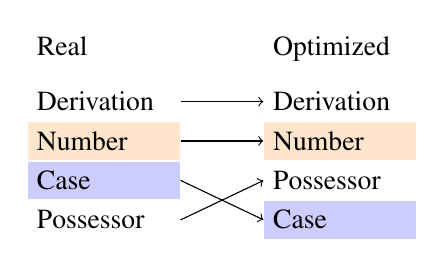
\begin{tikzpicture}[%
% common options for blocks:
block/.style = {draw, fill=blue!30, align=center, anchor=west,
            minimum height=0.65cm, inner sep=0},
% common options for the circles:
ball/.style = {circle, draw, align=center, anchor=north, inner sep=0}]
\node[rectangle,text width=1.7cm,anchor=base] (A0) at (1,-0.3) {Real};
\node[rectangle,text width=1.7cm,anchor=base] (B0) at (4,-0.3) {Optimized};
\node[rectangle,text width=1.7cm,anchor=base] (A1) at (1,-1.0) {Derivation};
\node[rectangle,text width=1.7cm,anchor=base, fill=orange!20] (A2) at (1,-1.5) {Number};
\node[rectangle,text width=1.7cm,anchor=base, fill=blue!20] (A3) at (1,-2.0) {Case};
\node[rectangle,text width=1.7cm,anchor=base] (A4) at (1,-2.5) {Possessor};
\node[rectangle,text width=1.7cm,anchor=base] (B1) at (4,-1.0) {Derivation};
\node[rectangle,text width=1.7cm,anchor=base, fill=orange!20] (B2) at (4,-1.5) {Number};
\node[rectangle,text width=1.7cm,anchor=base] (B3) at (4,-2.0) {Possessor};
\node[rectangle,text width=1.7cm,anchor=base, fill=blue!20] (B4) at (4,-2.5) {Case};
\draw[->] (A1.east) to (B1.west);
\draw[->] (A2.east) to (B2.west);
\draw[->] (A3.east) to (B4.west);
\draw[->] (A4.east) to (B3.west);
\end{tikzpicture}

  \end{minipage}
  \end{tabular}
  
    \caption{Real and optimized ordering (nouns)}
    \label{tab:my_label}
\end{figure}


\begin{figure}[]

\begin{tabular}{cccccccc}
\textbf{Turkish} & \textbf{Hungarian} & \textbf{Finnish} \\
\begin{minipage}{.3\textwidth}
    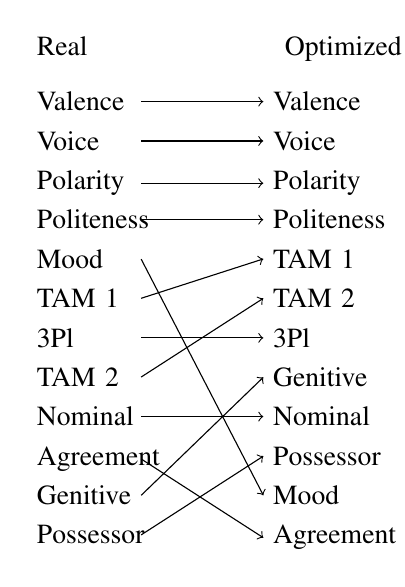
\begin{tikzpicture}[%
% common options for blocks:
block/.style = {draw, fill=blue!30, align=center, anchor=west,
            minimum height=0.65cm, inner sep=0},
% common options for the circles:
ball/.style = {circle, draw, align=center, anchor=north, inner sep=0}]
\node[rectangle,text width=1.2cm,anchor=base] (A0) at (1,-0.3) {Real};
\node[rectangle,text width=0.9cm,anchor=base] (B0) at (4,-0.3) {Optimized};
\node[rectangle,text width=1.2cm,anchor=base] (A1) at (1,-1.0) {Valence};
\node[rectangle,text width=1.2cm,anchor=base] (A2) at (1,-1.5) {Voice};
\node[rectangle,text width=1.2cm,anchor=base] (A3) at (1,-2.0) {Polarity};
\node[rectangle,text width=1.2cm,anchor=base] (A4) at (1,-2.5) {Politeness};
\node[rectangle,text width=1.2cm,anchor=base] (A5) at (1,-3.0) {Mood};
\node[rectangle,text width=1.2cm,anchor=base] (A6) at (1,-3.5) {TAM 1};
\node[rectangle,text width=1.2cm,anchor=base] (A7) at (1,-4.0) {3Pl};
\node[rectangle,text width=1.2cm,anchor=base] (A8) at (1,-4.5) {TAM 2};
\node[rectangle,text width=1.2cm,anchor=base] (A9) at (1,-5.0) {Nominal};
\node[rectangle,text width=1.2cm,anchor=base] (A10) at (1,-5.5) {Agreement};
\node[rectangle,text width=1.2cm,anchor=base] (A11) at (1,-6.0) {Genitive};
\node[rectangle,text width=1.2cm,anchor=base] (A12) at (1,-6.5) {Possessor};
\node[rectangle,text width=1.2cm,anchor=base] (B1) at (4,-1.0) {Valence};
\node[rectangle,text width=1.2cm,anchor=base] (B2) at (4,-1.5) {Voice};
\node[rectangle,text width=1.2cm,anchor=base] (B3) at (4,-2.0) {Polarity};
\node[rectangle,text width=1.2cm,anchor=base] (B4) at (4,-2.5) {Politeness};
\node[rectangle,text width=1.2cm,anchor=base] (B5) at (4,-3.0) {TAM 1};
\node[rectangle,text width=1.2cm,anchor=base] (B6) at (4,-3.5) {TAM 2};
\node[rectangle,text width=1.2cm,anchor=base] (B7) at (4,-4.0) {3Pl};
\node[rectangle,text width=1.2cm,anchor=base] (B8) at (4,-4.5) {Genitive};
\node[rectangle,text width=1.2cm,anchor=base] (B9) at (4,-5.0) {Nominal};
\node[rectangle,text width=1.2cm,anchor=base] (B10) at (4,-5.5) {Possessor};
\node[rectangle,text width=1.2cm,anchor=base] (B11) at (4,-6.0) {Mood};
\node[rectangle,text width=1.2cm,anchor=base] (B12) at (4,-6.5) {Agreement};
\draw[->] (A1.east) to (B1.west);
\draw[->] (A2.east) to (B2.west);
\draw[->] (A3.east) to (B3.west);
\draw[->] (A4.east) to (B4.west);
\draw[->] (A5.east) to (B11.west);
\draw[->] (A6.east) to (B5.west);
\draw[->] (A7.east) to (B7.west);
\draw[->] (A8.east) to (B6.west);
\draw[->] (A9.east) to (B9.west);
\draw[->] (A10.east) to (B12.west);
\draw[->] (A11.east) to (B8.west);
\draw[->] (A12.east) to (B10.west);
\end{tikzpicture}

  \end{minipage}
  &
  \begin{minipage}{.3\textwidth}
    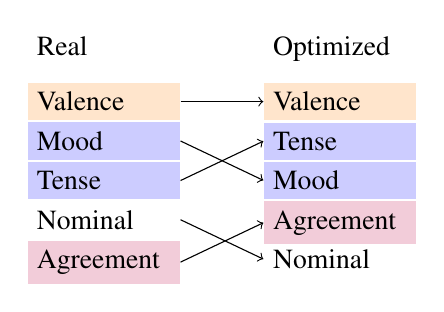
\begin{tikzpicture}[%
% common options for blocks:
block/.style = {draw, fill=blue!30, align=center, anchor=west,
            minimum height=0.65cm, inner sep=0},
% common options for the circles:
ball/.style = {circle, draw, align=center, anchor=north, inner sep=0}]
\node[rectangle,text width=1.7cm,anchor=base] (A0) at (1,-0.3) {Real};
\node[rectangle,text width=1.7cm,anchor=base] (B0) at (4,-0.3) {Optimized};
\node[rectangle,text width=1.7cm,anchor=base, fill=orange!20] (A1) at (1,-1.0) {Valence};
\node[rectangle,text width=1.7cm,anchor=base, fill=blue!20] (A2) at (1,-1.5) {Mood};
\node[rectangle,text width=1.7cm,anchor=base, fill=blue!20] (A3) at (1,-2.0) {Tense};
\node[rectangle,text width=1.7cm,anchor=base] (A4) at (1,-2.5) {Nominal};
\node[rectangle,text width=1.7cm,anchor=base, fill=purple!20] (A5) at (1,-3.0) {Agreement};
\node[rectangle,text width=1.7cm,anchor=base, fill=orange!20] (B1) at (4,-1.0) {Valence};
\node[rectangle,text width=1.7cm,anchor=base, fill=blue!20] (B2) at (4,-1.5) {Tense};
\node[rectangle,text width=1.7cm,anchor=base, fill=blue!20] (B3) at (4,-2.0) {Mood};
\node[rectangle,text width=1.7cm,anchor=base, fill=purple!20] (B4) at (4,-2.5) {Agreement};
\node[rectangle,text width=1.7cm,anchor=base] (B5) at (4,-3.0) {Nominal};
\draw[->] (A1.east) to (B1.west);
\draw[->] (A2.east) to (B3.west);
\draw[->] (A3.east) to (B2.west);
\draw[->] (A4.east) to (B5.west);
\draw[->] (A5.east) to (B4.west);
\end{tikzpicture}

  \end{minipage}
  &
    \begin{minipage}{.3\textwidth}
    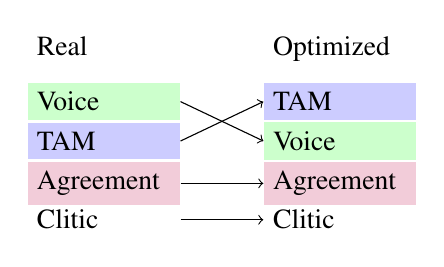
\begin{tikzpicture}[%
% common options for blocks:
block/.style = {draw, fill=blue!30, align=center, anchor=west,
            minimum height=0.65cm, inner sep=0},
% common options for the circles:
ball/.style = {circle, draw, align=center, anchor=north, inner sep=0}]
\node[rectangle,text width=1.7cm,anchor=base] (A0) at (1,-0.3) {Real};
\node[rectangle,text width=1.7cm,anchor=base] (B0) at (4,-0.3) {Optimized};
\node[rectangle,text width=1.7cm,anchor=base, fill=green!20] (A1) at (1,-1.0) {Voice};
\node[rectangle,text width=1.7cm,anchor=base, fill=blue!20] (A2) at (1,-1.5) {TAM};
\node[rectangle,text width=1.7cm,anchor=base, fill=purple!20] (A3) at (1,-2.0) {Agreement};
\node[rectangle,text width=1.7cm,anchor=base] (A4) at (1,-2.5) {Clitic};
\node[rectangle,text width=1.7cm,anchor=base, fill=blue!20] (B1) at (4,-1.0) {TAM};
\node[rectangle,text width=1.7cm,anchor=base, fill=green!20] (B2) at (4,-1.5) {Voice};
\node[rectangle,text width=1.7cm,anchor=base, fill=purple!20] (B3) at (4,-2.0) {Agreement};
\node[rectangle,text width=1.7cm,anchor=base] (B4) at (4,-2.5) {Clitic};
\draw[->] (A1.east) to (B2.west);
\draw[->] (A2.east) to (B1.west);
\draw[->] (A3.east) to (B3.west);
\draw[->] (A4.east) to (B4.west);
\end{tikzpicture}

  \end{minipage}
  \\
  \textbf{Korean}  & \textbf{Japanese} & \textbf{Sesotho} \\
      \begin{minipage}{.3\textwidth}
    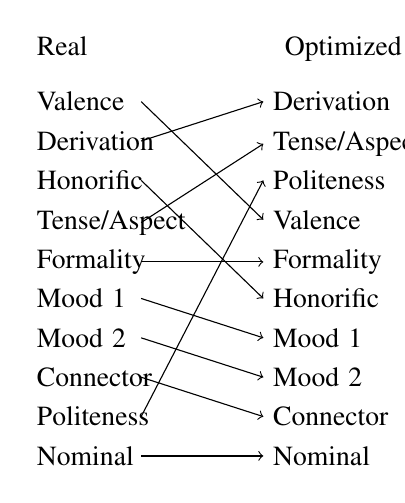
\begin{tikzpicture}[%
% common options for blocks:
block/.style = {draw, fill=blue!30, align=center, anchor=west,
            minimum height=0.65cm, inner sep=0},
% common options for the circles:
ball/.style = {circle, draw, align=center, anchor=north, inner sep=0}]
\node[rectangle,text width=1.2cm,anchor=base] (A0) at (1,-0.3) {Real};
\node[rectangle,text width=0.9cm,anchor=base] (B0) at (4,-0.3) {Optimized};
\node[rectangle,text width=1.2cm,anchor=base] (A1) at (1,-1.0) {Valence};
\node[rectangle,text width=1.2cm,anchor=base] (A2) at (1,-1.5) {Derivation};
\node[rectangle,text width=1.2cm,anchor=base] (A3) at (1,-2.0) {Honorific};
\node[rectangle,text width=1.2cm,anchor=base] (A4) at (1,-2.5) {Tense/Aspect};
\node[rectangle,text width=1.2cm,anchor=base] (A5) at (1,-3.0) {Formality};
\node[rectangle,text width=1.2cm,anchor=base] (A6) at (1,-3.5) {Mood 1};
\node[rectangle,text width=1.2cm,anchor=base] (A7) at (1,-4.0) {Mood 2};
\node[rectangle,text width=1.2cm,anchor=base] (A8) at (1,-4.5) {Connector};
\node[rectangle,text width=1.2cm,anchor=base] (A9) at (1,-5.0) {Politeness};
\node[rectangle,text width=1.2cm,anchor=base] (A10) at (1,-5.5) {Nominal};
\node[rectangle,text width=1.2cm,anchor=base] (B1) at (4,-1.0) {Derivation};
\node[rectangle,text width=1.2cm,anchor=base] (B2) at (4,-1.5) {Tense/Aspect};
\node[rectangle,text width=1.2cm,anchor=base] (B3) at (4,-2.0) {Politeness};
\node[rectangle,text width=1.2cm,anchor=base] (B4) at (4,-2.5) {Valence};
\node[rectangle,text width=1.2cm,anchor=base] (B5) at (4,-3.0) {Formality};
\node[rectangle,text width=1.2cm,anchor=base] (B6) at (4,-3.5) {Honorific};
\node[rectangle,text width=1.2cm,anchor=base] (B7) at (4,-4.0) {Mood 1};
\node[rectangle,text width=1.2cm,anchor=base] (B8) at (4,-4.5) {Mood 2};
\node[rectangle,text width=1.2cm,anchor=base] (B9) at (4,-5.0) {Connector};
\node[rectangle,text width=1.2cm,anchor=base] (B10) at (4,-5.5) {Nominal};
\draw[->] (A1.east) to (B4.west);
\draw[->] (A2.east) to (B1.west);
\draw[->] (A3.east) to (B6.west);
\draw[->] (A4.east) to (B2.west);
\draw[->] (A5.east) to (B5.west);
\draw[->] (A6.east) to (B7.west);
\draw[->] (A7.east) to (B8.west);
\draw[->] (A8.east) to (B9.west);
\draw[->] (A9.east) to (B3.west);
\draw[->] (A10.east) to (B10.west);
\end{tikzpicture}

  \end{minipage}
  &
  \begin{minipage}{.3\textwidth}
    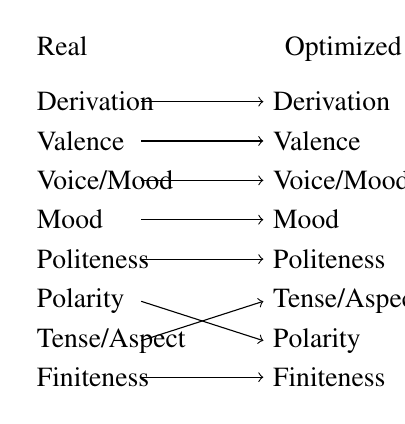
\begin{tikzpicture}[%
% common options for blocks:
block/.style = {draw, fill=blue!30, align=center, anchor=west,
            minimum height=0.65cm, inner sep=0},
% common options for the circles:
ball/.style = {circle, draw, align=center, anchor=north, inner sep=0}]
\node[rectangle,text width=1.2cm,anchor=base] (A0) at (1,-0.3) {Real};
\node[rectangle,text width=0.9cm,anchor=base] (B0) at (4,-0.3) {Optimized};
\node[rectangle,text width=1.2cm,anchor=base] (A1) at (1,-1.0) {Derivation};
\node[rectangle,text width=1.2cm,anchor=base] (A2) at (1,-1.5) {Valence};
\node[rectangle,text width=1.2cm,anchor=base] (A3) at (1,-2.0) {Voice/Mood};
\node[rectangle,text width=1.2cm,anchor=base] (A4) at (1,-2.5) {Mood};
\node[rectangle,text width=1.2cm,anchor=base] (A5) at (1,-3.0) {Politeness};
\node[rectangle,text width=1.2cm,anchor=base] (A6) at (1,-3.5) {Polarity};
\node[rectangle,text width=1.2cm,anchor=base] (A7) at (1,-4.0) {Tense/Aspect};
\node[rectangle,text width=1.2cm,anchor=base] (A8) at (1,-4.5) {Finiteness};
\node[rectangle,text width=1.2cm,anchor=base] (B1) at (4,-1.0) {Derivation};
\node[rectangle,text width=1.2cm,anchor=base] (B2) at (4,-1.5) {Valence};
\node[rectangle,text width=1.2cm,anchor=base] (B3) at (4,-2.0) {Voice/Mood};
\node[rectangle,text width=1.2cm,anchor=base] (B4) at (4,-2.5) {Mood};
\node[rectangle,text width=1.2cm,anchor=base] (B5) at (4,-3.0) {Politeness};
\node[rectangle,text width=1.2cm,anchor=base] (B6) at (4,-3.5) {Tense/Aspect};
\node[rectangle,text width=1.2cm,anchor=base] (B7) at (4,-4.0) {Polarity};
\node[rectangle,text width=1.2cm,anchor=base] (B8) at (4,-4.5) {Finiteness};
\draw[->] (A1.east) to (B1.west);
\draw[->] (A2.east) to (B2.west);
\draw[->] (A3.east) to (B3.west);
\draw[->] (A4.east) to (B4.west);
\draw[->] (A5.east) to (B5.west);
\draw[->] (A6.east) to (B7.west);
\draw[->] (A7.east) to (B6.west);
\draw[->] (A8.east) to (B8.west);
\end{tikzpicture}

  \end{minipage}
  \end{tabular}
  
  
    \caption{Real and optimized ordering (verbs)}
    \label{tab:my_label}
\end{figure}



\begin{figure}
 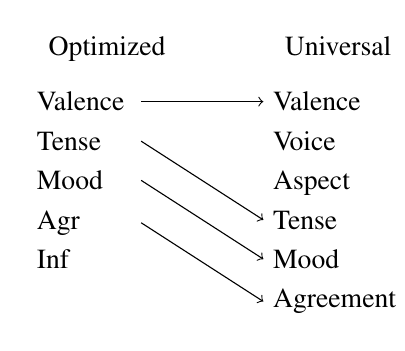
\begin{tikzpicture}[%
% common options for blocks:
block/.style = {draw, fill=blue!30, align=center, anchor=west,
            minimum height=0.65cm, inner sep=0},
% common options for the circles:
ball/.style = {circle, draw, align=center, anchor=north, inner sep=0}]
\node[rectangle,text width=0.9cm,anchor=base] (B0) at (4,-0.3) {Optimized};
\node[rectangle,text width=0.9cm,anchor=base] (C0) at (7,-0.3) {Universal};

\node[rectangle,text width=1.2cm,anchor=base] (B1) at (4,-1.0) {Valence};
\node[rectangle,text width=1.2cm,anchor=base] (B2) at (4,-1.5) {Tense};
\node[rectangle,text width=1.2cm,anchor=base] (B3) at (4,-2.0) {Mood};
\node[rectangle,text width=1.2cm,anchor=base] (B4) at (4,-2.5) {Agr};
\node[rectangle,text width=1.2cm,anchor=base] (B5) at (4,-3.0) {Inf};


\node[rectangle,text width=1.2cm,anchor=base] (C1) at (7,-1.0) {Valence};
\node[rectangle,text width=1.2cm,anchor=base] (C2) at (7,-1.5) {Voice};
\node[rectangle,text width=1.2cm,anchor=base] (C3) at (7,-2.0) {Aspect};
\node[rectangle,text width=1.2cm,anchor=base] (C4) at (7,-2.5) {Tense};
\node[rectangle,text width=1.2cm,anchor=base] (C5) at (7,-3.0) {Mood};
\node[rectangle,text width=1.2cm,anchor=base] (C6) at (7,-3.5) {Agreement};

\draw[->] (B1.east) to (C1.west);
\draw[->] (B2.east) to (C4.west);
\draw[->] (B3.east) to (C5.west);
\draw[->] (B4.east) to (C6.west);
\end{tikzpicture}

\begin{minipage}{.3\textwidth}
    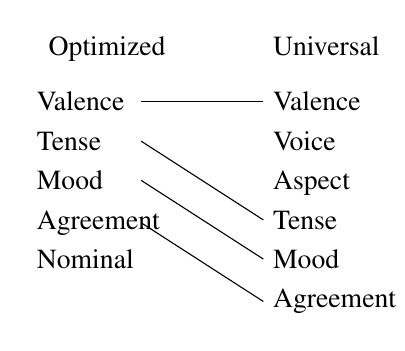
\begin{tikzpicture}[%
% common options for blocks:
block/.style = {draw, fill=blue!30, align=center, anchor=west,
            minimum height=0.65cm, inner sep=0},
% common options for the circles:
ball/.style = {circle, draw, align=center, anchor=north, inner sep=0}]
\node[rectangle,text width=1.2cm,anchor=base] (A0) at (4,-0.3) {Universal};
\node[rectangle,text width=0.9cm,anchor=base] (B0) at (1,-0.3) {Optimized};
\node[rectangle,text width=1.2cm,anchor=base] (A1) at (4,-1.0) {Valence};
\node[rectangle,text width=1.2cm,anchor=base] (A2) at (4,-1.5) {Voice};
\node[rectangle,text width=1.2cm,anchor=base] (A3) at (4,-2.0) {Aspect};
\node[rectangle,text width=1.2cm,anchor=base] (A4) at (4,-2.5) {Tense};
\node[rectangle,text width=1.2cm,anchor=base] (A5) at (4,-3.0) {Mood};
\node[rectangle,text width=1.2cm,anchor=base] (A6) at (4,-3.5) {Agreement};
\node[rectangle,text width=1.2cm,anchor=base] (B1) at (1,-1.0) {Valence};
\node[rectangle,text width=1.2cm,anchor=base] (B2) at (1,-1.5) {Tense};
\node[rectangle,text width=1.2cm,anchor=base] (B3) at (1,-2.0) {Mood};
\node[rectangle,text width=1.2cm,anchor=base] (B4) at (1,-2.5) {Agreement};
\node[rectangle,text width=1.2cm,anchor=base] (B5) at (1,-3.0) {Nominal};
\draw[-] (A1.west) to (B1.east);
\draw[-] (A4.west) to (B2.east);
\draw[-] (A5.west) to (B3.east);
\draw[-] (A6.west) to (B4.east);
\end{tikzpicture}

    \end{minipage}

    \caption{Caption}
    \label{fig:my_label}
\end{figure}


\section{Discussion}

We have examined morpheme order in nouns and verbs in six languages, testing the recently propiosed Efficient Tradeoff Hypothesis \citep{hahn2020modeling} as an explanatory account of morpheme ordering.
We compared actual morpheme orderings to other possible orderings and to orderings optimized for efficiency of the memory-surprisal tradeoff.
In most cases, we found that the real ordering provided more efficient tradeoffs than most alternative orderings.
More importantly, we found that the real orderings match the optimal orderings in many respects.
Ordering forms found in a corpus according according to real or optimized orderings yields the same orders in XXX of cases.
In some cases, particlarly for noun inflection, match between real and optimized orderings is perfect.

\subsection{Relation to previous accounts}

%\subsubsection{Semantic Scope; Syntactic Structure; Historical Development}

In this section, we discuss the linguistic literature on morpheme ordering.

\paragraph{Meaning and Scope}
As mentioned in section \becky{cite S2}, Bybee proposes a concept of \textit{semantic relevance}, which is the degree to which one morpheme affects the semantic content of the other \becky{cite bybee}. She hypothesizes that morphemes that are more highly relevant to each other should be closer to each other, and therefore proposes a universal ordering of verbal inflectional morphemes. For example, attaching a causative marker to a root meaning "to die" produces a verb form meaning "to kill." Since the causative greatly changes the semantic content of the original root, the causative is highly relevant to the root. 

\becky{Format Korean example of juk-da ``to die" and juk-i-da ``to kill"}

Bybee did not provide a way to computationally measure semantic relevance. However, our optimized orders of Turkish and Hungarian \becky{Are there other languages?} perfectly match Bybee's proposed universal verbal inflection order \becky{need a figure comparing optimized order to Bybee's order}. This suggests that high mutual information generally correlates with semantic relevance. 

Besides Bybee's account in terms of relevance, there are also accounts focusing on semantic scope \citep{rice2000morpheme}.

Also noted scope: \citep{baker1988incorporation,foley1984functional,chierchia1990meaning,valin1992a}



\paragraph{Morpheme Order and Word Order}
It has long been observed that the order of morphemes often parallels the order of independent words of corresponding meanings \citep{givon1971historical,venneman1973explanation,baker1985the}.
It has been argued that the order of morphemes reflects the order of formerly independent elements that have been fossilized into bound morphemes \citet{givon1971historical,venneman1973explanation}.
As the memory-surprisal tradeoff is optimized by word order, this is compatible with our results:
To the extent that morpheme order does reflect fossilized word order, morpheme order should continue to reflect optimization for the tradeoff.

On the other hand, \citet{bybee-morphology-1985} points out that there are historically documented cases where morpheme ordering has been restructured in ways that do not reflect former independent words, but respect the universal tendencies proposed by her (see also \citet{mithun2000the, haspelmath1993the, mithun1995affixation}; \citet[Section 15]{rice2000morpheme}).


\paragraph{Levels of Linguistic Description}
Besides the explanation of broad typological tendencies, which we are interested in here, the linguistic literature has also debated at which level of linguistic representation morpheme ordering should be described, proposing accounts located at different levels such as the syntax-phonology interface \citep{baker1985the} and an autonomous layer of morphological description \citep{hyman2003suffix}.
TODO also template vs scope vs...
We do not see the memory--surprisal tradeoff as competing with or contradicting these studies.
Rather, it specifies tendencies for ordering that could be implemented at different levels of linguistic description.




%One family of explanations holds that those affixes are closest to the root that are most relevant to the root \citep{bybee-morphology-1985}.
%Other explanations suggest that morphemes are ordered based on (TODO CITE).
%The most straightforwardly related account is that of Bybee (1985) Semantic relevance
%CARP template in Bantu
%Explanations for the orders
%A related, though different, account is in terms of semantic scope \cite{rice2000morpheme}.
%The scope hypothesis is attractive for some morphemes.
%For instance, 
%\cite{baker1985the} proposed the Mirror Principle, stating that the order of morphemes reflects ...
%This can be related to the scope-based explanation to the extent that syntactic structure and word order reflect scope.
%\cite{muysken1981quechua}
%\cite{mccarthy2008generalized} phonology
%\cite{hyman2003suffix}
%\cite{kanu2009suffix} morphotactics, not semantic scope


%\subsection{Relevance; Proximity; Iconicity}

%The relation  between mutual information and relevance

\subsection{Beyond Agglutionation}

Our study focused on agglutinatioon, where a word carries multiple clearly separated morphemes with distinct functions.
There are other types of morphological processes that deserve study.

While we have focused on the relative distance from the root, we have not touched on the question of why a morpheme is realized as a prefix or a suffix in a given language.
There are well-known correlations between suffixing or prefixing preference and word order \citep{greenberg1963universals}.

- infixation

Vowel change, productive in many languages and fossilized in English (swim $\rightarrow$ swam).

non-concatenative morphology (in Arabic, k-t-b `to write' forms katab- `wrote'. -aktub `write/be writing', -kutib- `was written').

\subsection{Limitations}

- genre of data: written



\section{Conclusion}

\bibliography{literature}
\bibliographystyle{natbib}
\appendix

\section{Appendix}



\subsection{Korean Verb Suffixes}

Korean verb morphology is very complex, and there is no generally agreed-upon description in terms of morphemes and slots.
We extracted suffixes based on the annotation found in the Kaist corpus and the linguistic literature on Korean \citep{yeon2010korean}.
The Kaist corpus provides segmentation into morphemes; we postprocessed it in two ways:
First, we made it more fine-grained by splitting morphemes that are merged in the annotation, and, second, we abstracted away consistently from allomorphy.
For instance, the Kaist corpus separately labels the segments \korean{ㅂ니다} \textit{-mnida} (as in \korean{합니다} \textit{hamnida} `does') and \korean{습니다} \textit{-seumnida} (as in \korean{했습니다} \textit{hatseumnida} `did').
These two segments actually are allomorphs, conditioned by the preceding material.
Furthermore, they can both be segmented into the formal marker \korean{ㅂ/습} (\textit{-p/-seup}, we label this underlying morpheme ``\textsc{p}$_5$'', see below for this notation), and the mood markers \korean{니} (\textit{-ni}, our \textsc{ni}$_6$) and \korean{다} (\textit{-da}, our \textsc{da}$_7$).
We therefore transform both segments into the abstract morpheme sequence \textsc{p}$_5$-\textsc{ni}$_6$-\textsc{da}$_7$ (see below for this notation).
We then partitioned the resulting morphemes into slots that make it possible to consistently describe the ordering of almost all forms encountered in the corpus.


With this procedure, we identified the nine slots described below. We show morphemes occurring at least 50 times in slots 2-8 in Figure~\ref{tab:korean-frequent-morphemes}.
We do not provide the list of conjunctive and nominalizing suffixes since these are very numerous.

Additional morphemes that occur less than X times are placed into an UNKNOWN slots, this affects X \% of morpheme occurrences in the dataset.
We indicate morphemes by a small-caps representation of a stylized phonological representation (such as \textsc{p} for -\korean{ㅂ/습}  -\textit{p/seup}),\footnote{These transcriptions are purely conventional, we do not intend these to correspond to a theory of how underlying phonological forms are realized as surface phone strings.} with a subscript indicating their slot (such as \textsc{p}$_5$-\textsc{ni}$_6$-\textsc{da}$_7$).

\begin{enumerate}
    \item Root
    %. The root may include a valency suffix, which is not separated frem the root in the dataset. We did not attempt to separate v
    \item Derivation: The two derivational suffixes are \textit{ha} (\citep[4.1.2]{yeon2010korean}) and the predicative \textit{i}, whose function is similar to that of a copula \citep[4.1.4]{yeon2010korean}.
    
    \item Honorific \textsc{si}$_3$ \citep[4.3.2, 4.4.1]{yeon2010korean}
    \item Tense/Aspect suffixes include -\textsc{ess}$_4$ for past \citep[4.5.1.1]{yeon2010korean}, -\textsc{essess}$_4$ for remote past \citep[4.5.1.2]{yeon2010korean}, -\textsc{get}$_4$ for future \citep[4.5.2.1]{yeon2010korean}
    \item Formality \textsc{p}$_5$ (allomorphs include -\textit{p}-, -\textit{m}-, -\textit{seum}-,  \citep[4.3.2]{yeon2010korean})
    \item We partition Mood suffixes into two slots. Frequent elements of the Mood I slot are -\textsc{n}-, -\textsc{ni}- \citep[4.3.2]{yeon2010korean}.
    
    \item Frequent elements of the Mood II slot are declarative -\textsc{da}- \citep[4.3.2]{yeon2010korean}, command -\textsc{ra}-, interrogative -\textsc{ka}-, the suffix  -\textsc{ji} \citep[4.2.2-3]{yeon2010korean}, and informal -\textsc{eo}- (informal).
    
    \item Polite -yo
    \item Conjunctive endings
    
    -go
    
    -seo
    
    and others
    
\end{enumerate}

TODO 

- Yeon 4.4.2.2 kkeo object honorific % 꺼

%\ex.\ag. oa di rek a \\
%\textsc{subject.agreement} \textsc{object.agreement} buy \textsc{indicative} \\
%`(he) is buying (it)'  \citep{demuth1992acquisition} \label{ex:oadireka}
%\bg. o pheh el a \\
%\textsc{subject.agreement} cook \textsc{applicative} \textsc{indicative} \\
%`(he) cooks (food) for (him)'  \citep{demuth1992acquisition}
%\label{ex:ophehela}


Examples:
\begin{tabular}{llllllllll}
1    & 3 & 4     & 5   & 6  & 7 & 8 \\
bara & sy & eots & eum & ni & da  & &  `wished'\\
wish & Honorific & Past & Formal & Indicative & Indicative \\
bara& & gess &  & &  eo & yo  &  `will wish' \\
wish  & &  Assertive && & informal & polite \\
\end{tabular}


Frequent morphemes:
\begin{table}
\resizebox{1.2\textwidth}{!}{
\begin{tabular}{llllllllll}
Slot & Morphs & Short & Freq. & Description & Citation \\ \hline\hline
Derivation & \korean{하} & HA$_2$ &	 68 & & \citep[4.1.2]{yeon2010korean}\\
& i & I$_2$ &	 3947 && \citep[4.1.4]{yeon2010korean} \\ \hline
Honorific & si 	& \textsc{si}$_3$ & 99 & &\citep[4.3.2, 4.4.1]{yeon2010korean}\\\hline
Tense/Asp. & \korean{었었} 	& ESSESS$_4$ &  56&& \citep[4.5.1.2]{yeon2010korean} \\
&get 	& GET$_4$ & 355 & assertive & \citep[4.5.2.1]{yeon2010korean}\\
& &ESS$_4$ &	 9720 & past& \citep[4.5.1.1]{yeon2010korean}\\\hline
Formality & p &P$_5$ &	 1761 & formal-polite &\citep[4.3.2]{yeon2010korean}\\\hline
Mood 1&ri & RI$_6$ &	 70 & I-guess-\\
&ni 	&NI$_6$ & 1700 && \citep[4.3.2]{yeon2010korean}\\
&n 	&N$_6$ &5069 & TODO  \\\hline
Mood 2&sida & SIDA$_7$ & 	 51 & Hortative, formal, polite \\
& \korean{어} 	& EO$_7$ & 62 & Indicative, informal\\
& \korean{자} & JA$_7$&	 163 & Hortative, formal, nonpolite & \citep[4.3.6.3]{yeon2010korean}\\
& \korean{소} &SO$_7$  &	 194 & See Table~\ref{tab:korean-styles} \\
& lkka & LKKA$_7$&	 200 & Interrogative & \citep[8.9]{yeon2010korean} \\
& \korean{오} & O$_7$ &	 226 & See Table~\ref{tab:korean-styles} \\
& ji & JI$_7$ &	 260 &    & \citep[4.2.2-3]{yeon2010korean}\\
& ka 	& KA$_7$ & 485 & Interrogative & \citep[4.3.4, p. 175; p. 183]{yeon2010korean} \\
& ra &RA$_7$ \korean{라} &	 959 & plain style command & \citep[4.3.6.4]{yeon2010korean} \\
& da & DA$_7$ &	 23035 & Declarative & \citep[4.3.2]{yeon2010korean} &  \\\hline
Polite & \korean{요} & YO$_8$&	 267 & See Table~\ref{tab:korean-styles} \\
\end{tabular}
}
\caption{Frequent Korean verb suffixes in slots 1-8.}\label{tab:korean-frequent-morphemes}
\end{table}

Infinitive -eo: -eora/-ara for imperative \citep[4.3.6.4]{yeon2010korean}


Next, we explain how our segmentation corresponds to commonly described paradigms.
First, in Table~\ref{tab:korean-styles}, we describe the correspondence to the speech style system described by \citep[4.3.2]{yeon2010korean}.
Second, in Tables~\ref{tab:korean-hada-1}--\ref{tab:korean-hada-3}, we show the paradigm for the verb \korean{하다} \textit{hada} `to do' as described in Wiktionary.\footnote{ \texttt{https://en.wiktionary.org/wiki/\korean{하다}} (retrieved Septemgber 16, 2020).}
In Table~\ref{tab:kroean-itda}, we show the part of the paradigm of the verb \textit{ida} `to be' corresponding to Table~\ref{tab:korean-hada-1} (the other parts of the paradigm are analogous to those of \textit{hada}).
Note that none of these paradigms are intended to be exhaustive lists of all forms of these verbs; instead, they represent commonly used forms in a systematic paradigmatic representation.


\begin{table}
\begin{tabular}{l||l|l|l|llll}
            & Statement & Question  & Command    & Proposal    \\ \hline\hline
Formal      &  \korean{ㅂ니다} & \korean{ㅂ니까} & \korean{지-ㅂ-지오} & \korean{지-ㅂ-지다} \\ 
      &  -mnida & -mnikka  & -sipsio & -sipsida  \\ 
      &  -P$_5$-NI$_6$-DA$_7$ & -P$_5$-NI$_6$-KKA$_7$  & -SI-P$_5$-SIO$_7$ & -SI$_3$-P$_5$-SIDA$_7$ \\ \hline
Polite      &  \multicolumn{4}{c}{\korean{아/어/요}}  \\
      &  \multicolumn{4}{c}{-a/eoyo}  \\
            & \multicolumn{4}{c}{-\textsc{eo}$_7$-\textsc{eo}$_8$} \\ \hline
Semi-Formal & \korean{오/소}   &           &   \korean{오}       &  \korean{-ㅂ-지다} \\
&  -o/so   &           & -o        & -p-sida \\
 &  -O$_7$/-SO$_7$   &           & -O$_7$    & -P$_5$-SIDA$_7$ \\\hline
Familiar    &    \korean{네}    &  \korean{나/는가} &  \korean{게}      &    \korean{세} \\
            & -ne                  & -na/neunka & -ge & -se \\ 
            & -NE$_7$                  & -NA$_7$/-NEUNKA$_7$ & -GE$_9$ & \textcolor{red}{-SE} \\ \hline
Intimate      &  \multicolumn{4}{c}{\korean{아/어}}  \\
      &  \multicolumn{4}{c}{-a/eo}  \\
            & \multicolumn{4}{c}{-\textsc{eo}$_7$} \\ \hline
Plain       &   \korean{다}     &  \korean{(느)냐} &  \korean{라}     &  \korean{자}\\
            &  -da    &  -(neu)nya & -ra      & -ja \\
            & -DA$_7$    &   -NYA$_7$          & -RA$_7$      & -JA$_7$\\
\end{tabular}
\caption{Correspondence between our morpheme segmentation and the speech style system described by \citep[4.3.2]{yeon2010korean}. In each cell, we provide the Hangul ending given by \citep{yeon2010korean}, a transliteration, and a representation in terms of underlying morphemes.}\label{tab:korean-styles}
\end{table}



\begin{table}
\begin{tabular}{llllllllll}
           &          &Formal non-polite & Informal non-polite & Informal polite & Formal polite \\ \hline \hline
\multirow{6}{*}{Indicative} & \multirow{3}{*}{Non-past} & \korean{한다} & \korean{해}  & \korean{해요}  & \korean{합니다}  \\
           &          & handa & hae & haeyo &  hamnida \\
           &          & -N$_6$-DA$_7$ & -EO$_7$ & -EO$_7$-YO$_8$ &  -P$_5$-NI$_6$-DA$_7$ \\
           &          & \korean{하+ㄴ다}  & \korean{하+어}    & \korean{하+어+요} & \korean{하+ㅂ니다} \\
            &          &  px+ef        &   pvg+ecs        & pvg+ef+jxf & pvg+ef\\
           \hline
           & \multirow{3}{*}{Past}     & \korean{했다}  & \korean{했어} & \korean{했어요}   & \korean{했습니다}  \\
           &      & haet-da &  haesseo &  haesseoyo  & haetseumnida \\
           &      & -ESS$_4$-DA &  -ESS$_4$-EO$_7$ &  -ESS$_4$-EO$_7$-YO$_8$  & -ESS$_4$-P$_5$-NI$_6$-DA$_7$ \\
           &      &  \korean{하+었+다}  &  \korean{하+었+어} & \korean{하+었+어+요} & \korean{하+었+습니다}  \\
           &      &  ncpa+xsv+ep+ef   & px+ep+ef   &   px+ep+ef+jxf &     pvg+ep+ef\\
           \hline
\multirow{6}{*}{Interrogative} & \multirow{3}{*}{Non-past} & \korean{하느냐} & \korean{해}  & \korean{해요}  & \korean{합니까} \\
 &  & haneunya &  hae &  haeyo & hamnikka\\
 &  & -NEUNYA$_7$ &  -EO$_7$ &  -EO$_7$-YO$_8$ & -P$_5$-NIKKA$_7$ \\
               && \korean{하+느냐} & & & \korean{하+ㅂ니까}    \\
              && px+ef & & & px+ef \\
 \hline
              & \multirow{3}{*}{Past} & \korean{했느냐} & \korean{했어} & \korean{했어요} & \korean{했습니까} \\
              &  & ha-n-neunya &  hae-sseo &  hae-sseo-yo &  haetseumnikka\\
              &  & -ESS$_4$-NEUNYA$_7$ &  -ESS$_4$-EO$_7$ &  -ESS$_4$-EO$_7$+YO$_8$ &  -ESS$_4$-P$_5$-NIKKA$_7$\\
              &  &  \korean{하+었+느냐}  & \korean{하+었+어} & \korean{하+었+어+요} & \korean{하+었+습니까} \\
              &  & +ep+ef  & +ep+ef            & px+ep+ef+jxf & pvg+ep+ef \\
              \hline
Hortative   && \korean{하자}  & \korean{해}  & \korean{해요}  & \korean{합시다}  \\
   && haja &  hae &  haeyo & hapsida \\
   && -JA$_7$ &  -EO$_7$ &  -EO$_7$-YO$_8$ & -P$_5$-SIDA$_7$ \\
   && \korean{+자} && \korean{하+어+요} & \korean{하+ㅂ시다}\\
   && +ef  && pvg+ef+jxf & ef \\
   \hline
Imperative  && \korean{해라, 하여라}  & \korean{해}  & \korean{해요}  & \korean{합시오}  \\
  && haera, hayeora &  hae &  haeyo &  hapsio \\
  && -EORA$_7$ & -EO$_7$ & -EO$_7$-YO$_8$ & -P$_5$-SIO \\
  && \korean{하+어라}, \korean{하+어라}  &  &    & \korean{+ㅂ시오} \\
  && pvg+ef,  pvg+ef                     &  &    &  +ef\\
  \hline
Assertive   && \korean{하겠다}  & \korean{하겠어}  & \korean{하겠어요}  & \korean{하겠습니다}  \\
   &&  hagetda & hagesseo &  hagesseoyo & hagetseumnida \\
   &&  -GESS$_4$-DA$_7$ & -GESS$_4$-EO$_7$ &  -GESS$_4$-EO$_7$-YO$_8$ & GESS$_4$-P$_5$-NI$_6$-DA$_7$ \\
&& \korean{하+겠+다}  & \korean{하+겠+어}   & \korean{하+겠+어+요} & \korean{하+겠+습니다}\\
&&  px+ep+ef          & pvg+ep+ef   & pvg+ep+ef+jxf & pvg+ep+ef\\
\hline
\end{tabular}
	\caption{Correspondence between our morpheme segmentation and the paradigm of \textit{hada} `to do' as described by Wiktionary and in the Kaist treebank. In each cell, we provide the Hangul (e.g., \korean{한다}) and transliterated (e.g., handa) forms given by Wiktionary, a representation in terms of underlying morphemes (e.g., -N$_6$-DA$_7$), and -- where available -- how the form is segmented in the Kaist corpus (e.g., \korean{하+ㄴ다} and px+ef).}\label{tab:korean-hada-1}
\end{table}

\begin{table}
\begin{tabular}{llllllllll}
           &          &Formal non-polite & Informal non-polite & Informal polite & Formal polite \\ \hline \hline
Cause/Reason && \korean{해} & \korean{해서, 하여서} & \korean{하니} & \korean{하니까} \\
&& hae & haeseo, hayeoseo & hani & hanikka \\ 
&& -EO$_7$ & -EOSEO$_9$ & -NI$_9$ & -NIKKA$_9$ \\
&& &\korean{하+어서, 하+어서} & \korean{하+니} & \korean{하+니까} \\
&& & pvg+ecs, xsm+ecs         & pvg+ecs & xsm+ef \\
\hline
Contrast && \korean{하지만} & \korean{하는데} & \korean{하더니} \\
 && hajiman & haneunde & haedoni & \\ 
 && -JIMAN$_9$ & -NEUNDE$_9$ & -DEONI$_9$ & \\ \hline
Conjunction && \korean{하고} \\
 && hago \\ 
&& -GO$_9$ \\ \hline
Condition && \korean{하면} & \korean{해야, 하여야} \\
&& hamyeon & haeya, hayeoya \\
&& MYEON$_9$ & EOYA$_9$ \\ \hline
Motive && \korean{하려고} \\
 && haryeogo \\
&& -RYEOGO$_9$
\end{tabular}
	\caption{Continuation of Table~\ref{tab:korean-hada-1}: Forms of \textit{hada} with a conjunctive ending.}\label{tab:korean-hada-2}
\end{table}



\begin{table}[]
    \centering
    \begin{tabular}{llllllllllllllllllllllllll}
           &          &Formal non-polite & Informal non-polite & Informal polite & Formal polite \\ \hline \hline
\multirow{2}{*}{Indicative} & Non-past & \korean{하신다} & \korean{하셔} & \korean{하세요, 하셔요} & \korean{하십니다} \\
                           && -SI-N-DA & SI-EO & SI-EO-YO & SI-P-NI-DA \\
&& \korean{하+시+ㄴ다}       &   --   &    \korean{하+시+어+요}             &  \korean{하+시+ㅂ니다}        \\
\hline
&& \korean{하셨다} & \korean{하셨어} & \korean{하셨어요} & \korean{하셨습니다} \\
&& SI-ESS-DA & SI-ESS-EO & SI-ESS-EO-YO & SI-ESS-P-NI-DA \\
& & \korean{하+셨+다}       &  --    &        --        &  \korean{하+셨+습니다}       \\
\hline
\multirow{2}{*}{Interrogative} & Non-past & \korean{하시느냐} & \korean{하셔} & \korean{하세요, 하셔요} & \korean{하십니까} \\
&& SI-NEUNYA & SI-EO & SI-EO-YO & SI-P-NIKKA \\
& &   --     &   --   &   \korean{하+시+어+요}             &  --        \\
\hline
& Past & \korean{하셨느냐} & \korean{하셨어} & \korean{하셨어요} & \korean{하셨습니까} \\
&      & SI-ESS-NEUNYA & SI-ESS-EO          & SI-ESS-EO-YO & SI-ESS-P-NIKKA \\
& &        &      &                &          \\
\hline
\multirow{2}{*}{Imperative} && \korean{하시라} & \korean{하셔} & \korean{하세요} & \korean{하십시오} \\
&& -SI-RA & -SI-EO & -SI-EO-YO & -SI-P-SIO \\
&        &      & \korean{하+시+어+}               &   \korean{하+십시오}       \\
\hline
\multirow{2}{*}{Assertive} & & \korean{하시겠다} & \korean{하시겠어} & \korean{하시겠어요} & \korean{하시겠습니다} \\
&        &  -SI-GESS-DA     &  -SI-GESS-EO              &  -SI-GESS-EO-YO & -SI-GESS-P-NI-DA        \\
&& -- & -- & -- & -- \\
    \end{tabular}
    \caption{Continuation of Tables~\ref{tab:korean-hada-1}--\ref{tab:korean-hada-2}: Conjugation of hada with an honorific (\textsc{si}$_3$). We provide Hangul forms, morpheme sequences, and -- where available -- segmentations as given in the Kaist corpus.}
    \label{tab:korean-hada-3}
\end{table}

%itda \url{https://en.wiktionary.org/wiki/%EC%9E%88%EB%8B%A4#Korean}

\begin{table}[]
    \centering
    \begin{tabular}{llllllllllllllllllllllllllllllllll}
           &          &Formal non-polite & Informal non-polite & Informal polite & Formal polite \\ \hline \hline
    \multirow{6}{*}{Indicative}         & Non-past  & \korean{있다} & \korean{있어} & \korean{있어요} & \korean{있습니다} \\
         &  &  \korean{있+다} & \korean{있+어} & \korean{있+어+요} & \korean{있+습니다}\\
         &  &  -DA            & -EO            & -EO-YO            & -P-NI-DA \\
         &  & +ef & +ef & +ef+jxf & +ef \\
         \hline
 & Past & \korean{있었다} & \korean{있었어} & \korean{있었어요} & \korean{있었습니다} \\
         &  & \korean{있+었+다} & \korean{있+었+어} & \korean{있+었+어+요} & \korean{있+었+습니다}\\
         && -ESS-DA            & ESS-EO             & ESS-EO-YO & -ESS-P-NI-DA \\
         &  & +ep+ef & +ep+ef & +ep+ef+jxf & +ep+ef \\
         \hline
\multirow{6}{*}{Interrogative} & Non-past  & \korean{있느냐} & \korean{있어} & \korean{있어요} & \korean{있습니까} \\
&& -NEUNYA & -EO & -EO-YO & -P-NIKKA \\
         &  & \korean{있+느냐} & \korean{있+어} & \korean{있+어+요} & \korean{있+습니까}\\
         &  & +ef              & +ef  & +ef+jxf & +ef\\
         \hline
         & Past & \korean{있었느냐} & \korean{있었어} & \korean{있었어요} & \korean{있었습니까} \\
         && -ESS-NEUNYA & -ESS-EO & -ESS-EO-YO & -ESS-P-NIKKA \\
         &  & \korean{있+었+느냐} & \korean{있+었+어} & \korean{있+었+어+요}\\
         &  & +ep+ef & paa+ep+ef &  paa+ep+ef+jxf\\
         \hline
\multirow{3}{*}{Assertive} &  & \korean{있겠다} & \korean{있겠어} & \korean{있겠어요} & \korean{있겠습니다} \\
&& -GESS-DA & -GESS-EO & -GESS-EO-YO & -GESS-P-NI-DA \\
         &  & \korean{있+겠+다} & \korean{} & \korean{있+겠+어+요} & \korean{있+겠+습니다}\\
         &  & +ep+f             &           & paa+ep+ef+jxf & paa+ep+ef\\
    \end{tabular}
    \caption{Conjugation of itda}
    \label{tab:kroean-itda}
\end{table}



%\begin{longtable}{lllll}
%NOMINALIZER-future-determiner-\korean{을} & EUL &	 128 \\
%NOMINALIZER-topic?past-determiner-\korean{은} & EUN&	 129 \\
%NOMINALIZER-nominalizer-informal-nonpolite-gi & GI &	 151 \\
%NOMINALIZER-nominalizer-formal-nonpolite-m 	& M & 216 \\
%\end{longtable}


\subsection{Turkish Verb Suffixes}

In Table~\ref{tab:turkish-suffixes}, we show the list of identified Turkish verb suffixes.
In Figure~\ref{tab:turkish-yapmak}, we show how our segmentation corresponds to the paradigm of yapmak as described by Wiktionary.\footnote{From https://en.wiktionary.org/wiki/yapmak\#Turkish, retrieved September 5, 2020.}



\begin{table}
\resizebox{\textwidth}{!}{
\begin{tabular}{ll||llllllllllllll}
         &        & 1       & 2        & 3        & 1      & 2      & 3 \\ \hline\hline
 DNP & A & yaparım & yaparsın &  	yapar & yaparız & yaparsınız &  	yaparlar \\
                    &  & -AR-IM & -AR-SIN &  	-AR & -AR-IZ & -AR-SINIZ &  	-AR-LAR \\ \hline
                & I & yapıyorum & yapıyorsun & 	yapıyor &	yapıyoruz &	yapıyorsunuz &	yapıyorlar \\
                &  & -IYOR-UM & -IYOR-SUN & 	-IYOR &	-IYOR-UZ &	-IYOR-SINIZ &	-IYOR-LAR \\ \hline
                & Pr  & yapacağım &	yapacaksın 	& yapacak 	& yapacağız &	yapacaksınız &	yapacaklar \\ 
                &   & -ACAK-IM &	-ACAK-SIN 	& -ACAK 	& -ACAK-IZ &	-ACAK-SINIZ &	-ACAK-LAR \\ \hline\hline
        DP    & Pe &yaptım &	yaptın &	yaptı &	yaptık &	yaptınız &	yaptılar \\
              &  &-TI-IM &	-TI-SIN &	-TI &	-TI-K &	-TI-SINIZ &	-TI-LAR \\ \hline
                & I & yapıyordum &	yapıyordun &	yapıyordu &	yapıyorduk &	yapıyordunuz &	yapıyorlardı \\ 
                &  & -IYOR-DU-IM &	-IYOR-DU-SIN &	-IYOR-DU &	-IYOR-DU-K &	-IYOR-DU-SINIZ &	-IYOR-LAR-DU \\ \hline\hline
 I     & Pe & yapmışım &	yapmışsın &	yapmış &	yapmışız &	yapmışsınız &	yapmışlar \\
       &  & -MIS-IM &	-MIS-SIN &	-MIS &	-MIS-IZ &	-MIS-SINIZ &	-MIS-LAR \\ \hline
               & A & yaparmışım &	yaparmışsın &	yaparmış &	yaparmışız &	yaparmışsınız& 	yaparlarmış \\ 
            &  & -AR-MIS-IM &	-AR-MIS-SIN &	-AR-MIS &	-AR-MIS-IZ &	-AR-MIS-SINIZ& 	-AR-LAR-MIS \\ \hline
               & I & yapıyormuşum &	yapıyormuşsun &	yapıyormuş &	yapıyormuşuz &	yapıyormuşsunuz &	yapıyorlarmuş \\
               &              & -IYOR-MUS-IM &	-IYOR-MUS-SUN &	-IYOR-MUS &	-IYOR-MUS-UZ &	-IYOR-MUS-SUNUZ &	-IYOR-LAR-MUS \\
\end{tabular}
}
\caption{Turkish}\label{tab:turkish-yapmak}
\end{table}

\begin{table}
\begin{tabular}{llllllll}
\hline
Valence &   & Causative\\
\hline
Voice &   & Passive\\
\hline
Polite &   & \\
\hline
Polarity  & MA & Negation & \\
\hline
Mood \\
\hline
TAM1      & AR & Aorist, nonpast, direct \\
          & IYOR & Imperfective, direct & Aspect=Prog\\
          & ACAK & Prospective, nopast, direct\\
          & MIS1  & Perfective, indirect \\
          & TI & Perfective, past, direct \\
\hline
V Noun &  \\
\hline
3rd Plural& LAR & 3rd Plural\\
\hline
TAM2      & MUS2 & Aorist/Imperfective, indirect \\
          & DU & imperfective, past, direct \\
\hline
Agreement & IM & 1st singular\\
          & SIN &2nd singular\\
          & IZ  & 1st plural\\
          & SINIZ & 2nd plural \\
          & K     & 1st plural, past direct \\
\hline
Poss Num/Pers & \\
\hline
Gen & \\
\hline
\end{tabular}
\caption{Suffixes in Turkish}\label{tab:turkish-suffixes}
\end{table}




\subsection{Hungarian Verb Suffixes}


In Table~\ref{tab:hungarian-suffixes}, we show the list of identified Hungarian verb suffixes.
In Figure~\ref{tab:hungarian-paradigms}, we show how our segmentation corresponds to the paradigm of three verbs as described by Wiktionary.\footnote{From \texttt{https://en.wiktionary.org/wiki/tesz},
\texttt{https://en.wiktionary.org/wiki/csinál},
\texttt{https://en.wiktionary.org/wiki/ismer}, retrieved September 5, 2020.}





\begin{table}
    \centering
    \begin{tabular}{lllllllll}
    \hline
Valence	    & AT & Causative \\ \hline
Mood	    & HET & Potential \\
         & N & conditional \\
         & J & subjunctive \\
\hline
Tense& T & indicative past \\
         \hline
Finiteness  & NI & Infinitive \\
\hline
%Definiteness & I & definite 2/3pl \\
%         \hline
Agreement (Obj+Subj)         & EK & 1sg indefinite present\\
         & EL & 2sg present\\
         & UNK & 1pl present\\
         & TEK & 2pl\\
         & NEK & 3pl present\\
         & EM & 1sg past or definite \\
         & ED & 2sg definite \\
         \hline
    \end{tabular}
    \caption{Hungarian verb suffixes}
    \label{tab:hungarian-suffixes}
\end{table}

\begin{table}[]
    \centering
\resizebox{\textwidth}{!}{
    \begin{tabular}{lll||llllllllllllllll}
    &    & &  1 & 2 & 3 & 1 & 2 & 3 \\ \hline
Ind & Pres   &  I    & teszek &	teszel &	tesz &	teszünk &	tesztek &	tesznek \\
    &        &       & csinálok &	csinálsz &	csinál &	csinálunk &	csináltok &	csinálnak \\
   &&&  ismerek &	ismersz &	ismer &	ismerünk &	ismertek &	ismernek \\
 &    &      & -EK &	-EL &	- &	-UNK &	-TEK &	-NEK \\ \hline
   &&  D    & teszem &	teszed &	teszi &	tesszük &	teszitek &	teszik \\
   &&       & csinálom &	csinálod &	csinálja &	csináljuk &	csináljátok &	csinálják \\
  &&& ismerem &	ismered &	ismeri &ismerjük &	ismeritek &	ismerik \\
&&      & -EM &	-ED &	-I &	-I-UK &	-I-TEK &	-I-EK \\ \hline
   &&      & teszlek \\ \hline\hline
& Past &     I    &tettem &	tettél &	tett &	tettünk &	tettetek &	tettek \\
&      &          & csináltam &	csináltál &	csinált &	csináltunk &	csináltatok &	csináltak \\
&&&ismertem &	ismertél &	ismert &	ismertünk &	ismertetek &	ismertek \\
	    &  &         &-T-EM &	-T-EL &	-T &	-T-UNK &	-T-TEK &	-T-EK \\ \hline
 & &   D    &tettem &	tetted &	tette &	tettük &	tettétek &	tették \\
 & &        & csináltam &	csináltad &	csinálta &	csináltuk &	csináltátok &	csinálták \\
&&& ismertem &	ismerted &	ismerte &	ismertük &	ismertétek 	&ismerték \\
	    & &       &-T-EM &	-T-ED &	-T-I &	-T-UK &	-T-I-TEK &	-T-I-EK \\ \hline
  &&       &tettelek \\ \hline
Cond  &Pres &   I    &tennék &	tennél &	tenne &	tennénk &	tennétek &	tennének \\
      &     &        & csinálnék &	csinálnál &	csinálna &	csinálnánk 	&csinálnátok &	csinálnának \\
  &&&    ismernék &	ismernél &	ismerne &	ismernénk &	ismernétek &	ismernének \\
  & &   I    &-N-EK &	-N-EL &	-N &	-N-ENK &	-N-TEK &	-N-NEK \\\hline
   &&  D    &tenném &	tennéd &	tenné &	tennénk &	tennétek &	tennék \\
   &&       & csinálnám &	csinálnád &	csinálná &	csinálnánk &	csinálnátok &	csinálnák \\
 &&&  ismerném &	ismernéd &	ismerné &	ismernénk 	&ismernétek &	ismernék \\
&&      &-N-EM &	-N-ED &	-N-I &	-N-ENK &	-N-TEK &	-N-EK \\ \hline
       &&  &tennélek \\ \hline
Subj & Pres & I         &tegyek &	tégy or tegyél &	tegyen &	tegyünk &	tegyetek &	tegyenek \\
     &      &           & csináljak &	csinálj or
csináljál &	csináljon &	csináljunk& 	csináljatok &	csináljanak \\
&&&ismerjek &	ismerj or
ismerjél &	ismerjen &	ismerjünk &	ismerjetek &	ismerjenek \\
 &  &          &-J-EK &	-J or -J-EL &	-J-EN &	-J-UNK &	-J-TEK &	-J-NEK \\ \hline
&&D         &tegyem &	tedd or tegyed &	tegye &	tegyük& 	tegyétek &	tegyék \\
&&          & csináljam &	csináld or
csináljad &	csinálja &	csináljuk &	csináljátok &	csinálják \\
&&&ismerjem &	ismerd or
ismerjed &	ismerje &	ismerjük &	ismerjétek & ismerjék
 \\
&&         &-J-EM &	-ED or -J-ED &	-J-I &	-J-UK & 	-J-I-TEK &	-J-I-EK \\ \hline
  &&       &tegyelek \\
    \end{tabular}
    }
    \caption{Hungarian verb suffixes (tense, mood, definitiness, person/number).}
    \label{tab:hungarian-paradigms}
\end{table}


\subsection{Sesotho}

We describe Sesotho verb affixes following \cite{Hahn2020modeling}.
who described these based on \citep{doke1967textbook, guma1971outline, demuth1992acquisition}.
We refer to \cite{Hahn2020modeling} for further details.

\begin{enumerate}
    \item Subject agreement: This morpheme encodes agreement with the subject, for person, number, and noun class (the latter only in the 3rd person) \cite[\textsection 395]{doke1967textbook}.
            The annotation provided by \cite{demuth1992acquisition} distinguishes between ordinary subject agreement prefixes and agreement prefixes used in relative clauses; we distinguish these morpheme types here.

    \item Negation \citep[\textsection 429]{doke1967textbook}

    \item Tense/aspect marker   \citep[\textsection 400--424]{doke1967textbook}

    \item Object agreement or reflexive marker \citep[\textsection 459]{doke1967textbook}.
    Similar to subject agreement, object agreement denotes person, number, and noun class features of the object.
\end{enumerate}
We identified the following suffixes:

\begin{enumerate}
\item Semantic derivation: reversive (e.g., `do' $\rightarrow$ `undo')
\item Valence: (e.g., causative, neuter/stative, applicative, and reciprocal)
    \item Voice: passive
    \item Tense
    \item Mood
    \item Interrogative and relative markers
\end{enumerate}

\subsection{Japanese}

\paragraph{Japanese Verbs}
We describe Japanese verb suffixes following \citep{Hahn2020modeling}, who described these based on \citep{kaiser2013japanese,hasegawa2014japanese}.
We refer to \citep{Hahn2020modeling} for details.

\begin{enumerate}
\item \textit{suru}: obligatory suffix after Sino-Japanese words when they are used as verbs
\item Valence: causative (-\textit{ase}-)
\item Voice and Mood: passive (-\textit{are}-, -\textit{rare}-) and potential (-\textit{e}-, -\textit{are}-, -\textit{rare}-)
\item Politeness (-\textit{mas}-)
\item Mood: desiderative (-\textit{ta}-)
\item Negation (-\textit{n}-)
\item Tense, Aspect, Mood, and Finiteness: past (-\textit{ta}), future/hortative (-\textit{yoo}) \citep[229]{kaiser2013japanese}, nonfiniteness (-\textit{te})
\end{enumerate}



\end{document}





